\documentclass{report}

\usepackage[a4paper, left=2.5cm, right=2cm, top=1.5cm, bottom=2cm, includefoot=false, includehead=false]{geometry}
\usepackage[MeX]{polski}
\usepackage[utf8]{inputenc}
\usepackage{enumerate}
\usepackage{graphicx}
\usepackage{float}
\usepackage{verbatim}
\usepackage{url}

\makeatletter

\newcommand{\linia}{\rule{\linewidth}{0.4mm}}

\renewcommand{\maketitle}{\begin{titlepage}

    \vspace*{1cm}

    \begin{center}\small

    Politechnika Wrocławska\\

    Wydział Elektroniki W-4\\

    \end{center}

    \vspace{3cm}

    \noindent\linia

    \begin{center}

      \LARGE Projekt lokalne sieci komputerowe\\
      \normalsize\textsc{\@title}

         \end{center}

     \noindent\linia

    \vspace{0.5cm}

    \begin{flushright}

    \begin{minipage}{6cm}

    \textit{\small Autor:}\\

    \normalsize \textsc{\@author} \\

    \end{minipage}

    \vspace{5cm}

     {\small Prowadzący:}\\

         Dr hab. inż. Krzysztof Walkowiak

     \end{flushright}

    \vspace*{\stretch{6}}

    \begin{center}

    \@date

    \end{center}

  \end{titlepage}

}
\makeatother

\author{Mateusz Socha 181308 \\ Janusz Kuszczyński 184872 }

\title{}

\sloppy

\begin{document}

\maketitle
\tableofcontents

\chapter{Wstęp}

\vspace{0,5cm}
Projekt instalacji sieciowej jest realizowany dla firmy ComputerBudy. Siedziba która jest jednocześnie przedmiotem tego projektu znajduje się
przy ulicy Szwajcarska 22 w Wrocławiu.

\begin{figure}[H]
  \centering
      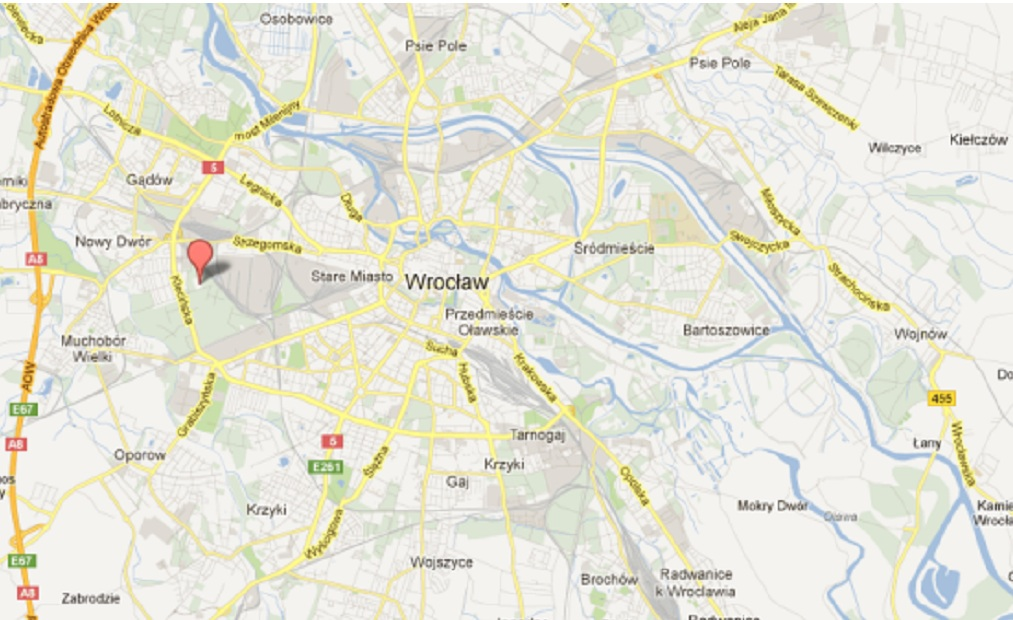
\includegraphics[width=0.8\textwidth]{./obrazki/adres_computerbudy.jpeg}
  \caption{Lokalizacja centrali firmy na mapie Wrocławia.}
\end{figure}

ComputerBudy jest firmą z działu IT. Zajmuje się ona zdalną pomocą przy problemach informatycznych. Zapewnia również zdalną administrację dla
skomplikowanych aplikacji na urządzeniach użytkownika. Jej oferta jest skierowana do osób prywatnych oraz małych i średnich firm, które
nie posiadają własnego działu IT.

Profil usług świadczonych powoduje, że brak połączenia z zewnętrzną siecią internet całkowicie paraliżuje całą firmę. 
Nawet awaria pojedynczego stanowiska powoduje straty. Restrykcyjna polityka bezpieczeństwa firmy sprawia, że nawiązanie połączenia z klientem
może nastąpić tylko z sieci firmowej. Aby zwiększyć bezpieczeństwo każde stanowisko obsługujące klientów jest przyłączone do sieci
za połączone za pomocą kabla UTP. Obostrzenia te spowodowane są obawą przed podsłuchaniem poufnych informacji przez osoby niepowołane oraz
przejęciem kontroli nad komputerem klienta podszywając się pod pracownika firmy z innej lokacji.

ComputerBudy wynajmuje łącznie 5 pięter w dwóch bliźniaczych budynkach stojących obok siebie.W pierwszym dwa i w następnym budynku kolejne 3.
Pozostałe piętra wynajmują inne firmy.

Celem naszej pracy jest stworzenie projektu nowej instalacji teleinformatycznej na użytkowanych przez firmę piętrach w obu budynkach.
\pagebreak[4]

 Zakres projektu:
\begin{itemize}
\item{Inwentaryzacja sprzętu i infrastruktury dostępnej w przedsiębiorstwie}
\item{Analiza potrzeb użytkowników – wymagania zamawiającego}
\item{Założenia projektowe}
\item{Projekt sieci}
\subitem{Projekt logiczny sieci wraz z opisem koncepcji rozwiązania}
\subitem{Konfiguracja adresacji IP}
\subitem{Projekt okablowania}
\subitem{Projekt podłączenia do Internetu}
\subitem{Analiza bezpieczeństwa i niezawodności sieci}
\subitem{Kosztorys urządzeń}
 
\end{itemize}
Wnioskując z profilu usług firmy priorytetowe znaczenie podczas projektowania należy nadać niezawodności. Drugim w kolejności czynnikiem jest oczywiście
szeroko pojęte bezpieczeństwo. Wskazane jest również zapewnienie łatwej możliwości rozbudowy sieci w tym budynku na kolejne piętra.
Oczywiście jako, że zleceniodawca jest firmą prywatną należy zminimalizować koszty całego przedsięwzięcia.

Do stworzenia projektu instalacji teleinformatycznej zostaną użyte szczegółowe plany budynków udostępnione przez zleceniodawcę.
Wymagania użytkowników zostaną opracowane na podstawie danych przekazanych przez administratora IT firmy oraz poprzez konsultację
z samymi pracownikami. Przepustowości łącz w nowej instalacji zostaną oszacowane na podstawie danych z obecnie istniejącej sieci komputerowej.

\chapter{Inwentaryzacja sprzętu i infrastruktury dostępnej w przedsiębiorstwie}
Na podstawie udostępnionej dokumentacji oraz wizyt w budynku mieszczącym firmę opracowano zestawienie zasobów obecnie posiadanych przez firmę.

\paragraph{Instalacja siecowa}



W obecnej architekturze sieciowej razem w obu budynkach znajduje się 290 gniazdek ethernetowych. Nie wszystkie są obecnie używane.
Całe obecna instalacja opera się na elementach z kategorii 3. Jest to wyraźnie przestarzała technologia. Starą instalacje należy zdemontować a 
odzyskane elementy sprzedać. Działania te ma wykonać firma instalacyjna.

\paragraph{Serwery w firmie}



W centrali znajdują się 2 serwery. Pierwszy realizuje usługę
bazy danych natomiast drugi hostuje stronę internetową firmy. Serwery działają pod kontrolą systemu NetWare. Znajdują się on w
pomieszczeniu nr 11 w budynku A. Pokój ten jest specjalnie przystosowany, posiada oddzielną klimatyzacje oraz jest 
dobrze zabezpieczone przed niepowołanym fizycznym dostępem. Takie samo pomieszczenie znajduje się w budynku B i ma również nr 11. Obecnie nie jest
używane. Właśnie w tych dwóch pomieszczeniach będą znajdować się urządzenia sieciowe oraz szafy krosownicze.

\paragraph{Sprzęt}


Wszystkie komputery PC oraz inne urządzenia przyłączone do sieci posiadają interfejsy sieciowe ethernet i spełniają wymagania niezbędne
do połączenia do nowej sieci. Nasz projekt nie obejmuje zakupu urządzeń końcowych dla użytkowników.

\paragraph{Programy} Spis programów używanych w firmie:
\begin{enumerate}
 \item system operacyjny Windows XP
 \item przeglądarka Firefox
 \item program pocztowy Thunderbird
 \item Skype dla firm
 \item edytor tekstu Microsoft Office
 \item klient NetWare
 \item ssh
 \item TeamViever
 \item program księgowo kadrowy Płatnik
\end{enumerate}

\paragraph{Opis budynków}Budynki w których firma ma swoją siedzibę to nowoczesne biurowce. Wynajmujący piętro sam zagospodarowuje większość 
znajdującej się tam przestrzeni za pomocą modułowej architektury boxów. Aby umożliwić dużą elastyczność konfiguracji przestrzennej piętra 
wyposażone są w podwieszane sufity w których poprowadzono jest większość instalacji. Właśnie pod kątem tego montażu zostanie zaprojektowany plan
okablowania.

\paragraph{Zasilanie}Sieć energetyczna zainstalowana w budynku spełnia wszelkie wymagania dotyczące bezpieczeństwa oraz wydajności wymaganej dla sieci komputerowej.
Warte odnotowania jest obecność instalacji piorunochronowej na obu budynkach. Znacząco zwiększa to bezpieczeństwo sprzętów elektronicznych zainstalowanych
w budynku.

\paragraph{Zakłócenia}Zakłócenia elektromagnetyczne w budynku są na tyle małe, że można je pominąć. W okolicy nie pracuje żaden duży zakład przemysłowy, który mógłby 
znacząco wpłynąć na parametry zasilania w sieci. Inne firmy, które prowadzą swoją działalność w tych budynkach korzystają jedynie z standardowego
sprzętu biurowego połączonego kablową siecią ethernetową. Brak innych sieci bezprzewodowych w budynkach znacząco ułatwia implementacje sieci wifi
ponieważ nie występuje problem interferencji międzykanałowych.


\pagebreak[4]
\section{Wymiary budynków}
%Plany budynków
\begin{figure}[H]
  \centering
      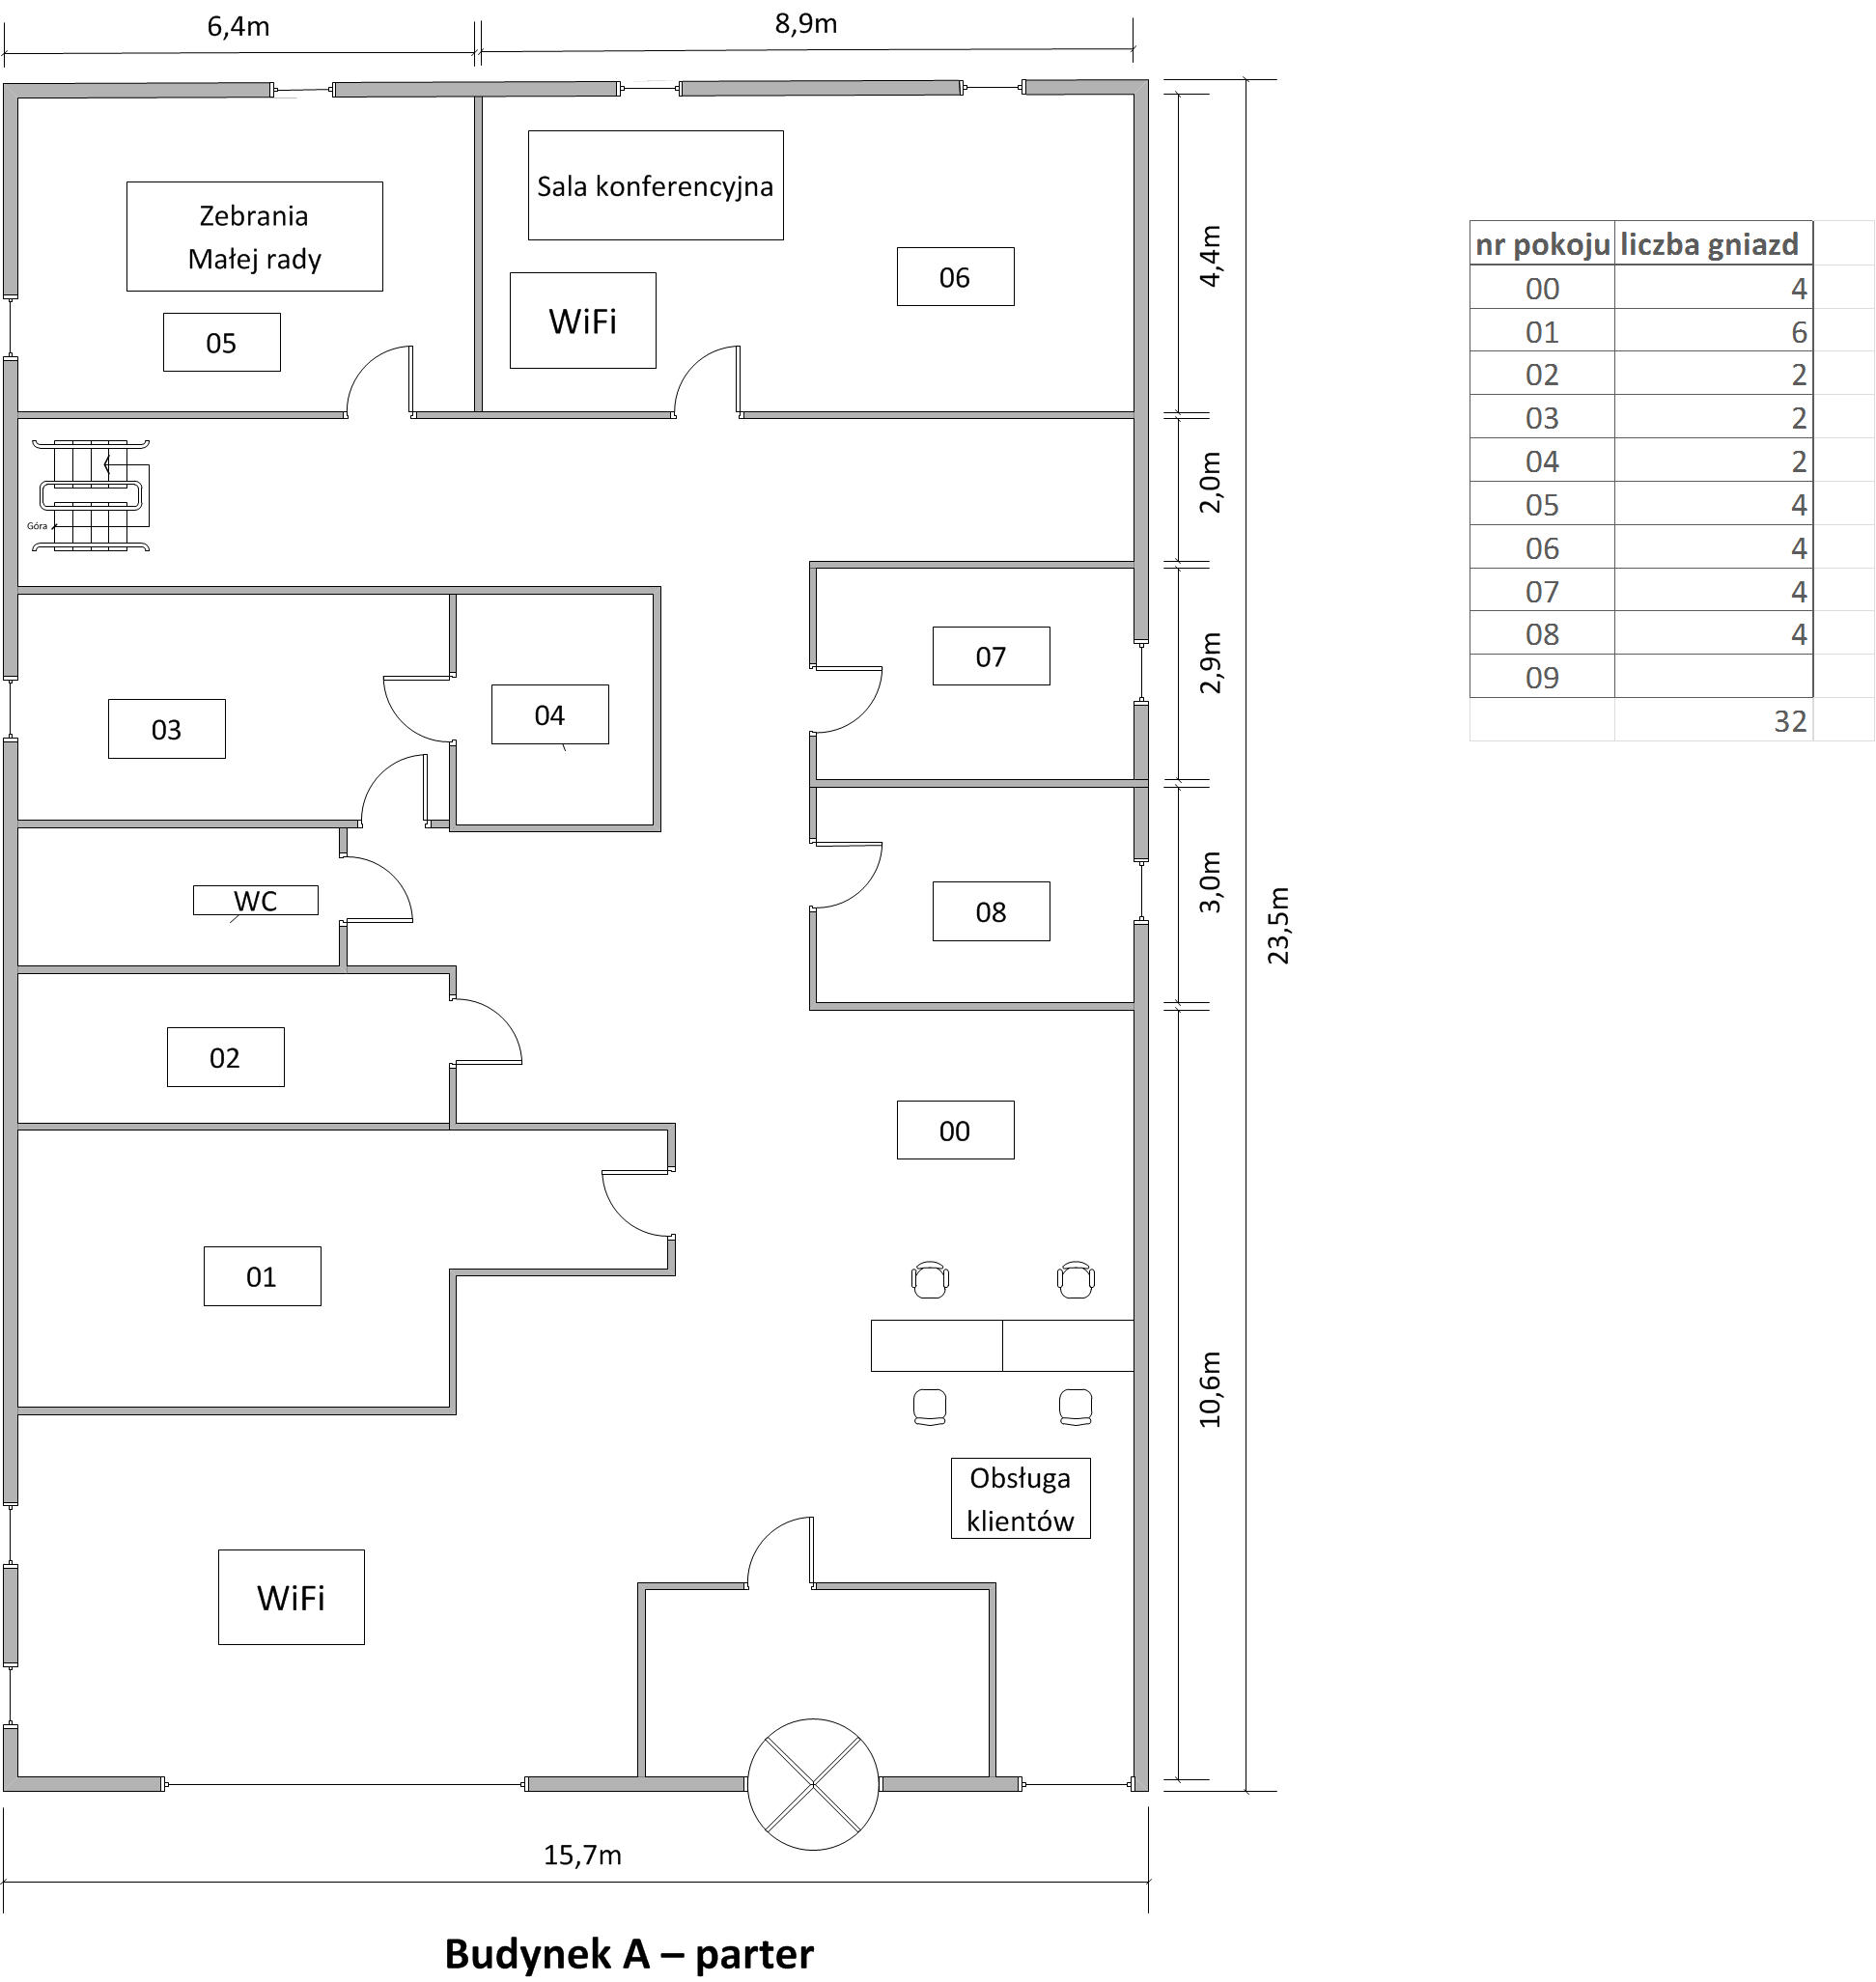
\includegraphics[width=\textwidth]{./obrazki/plany_wew/a0.png}
\end{figure}

\begin{comment}
\begin{figure}[H]
  \centering
      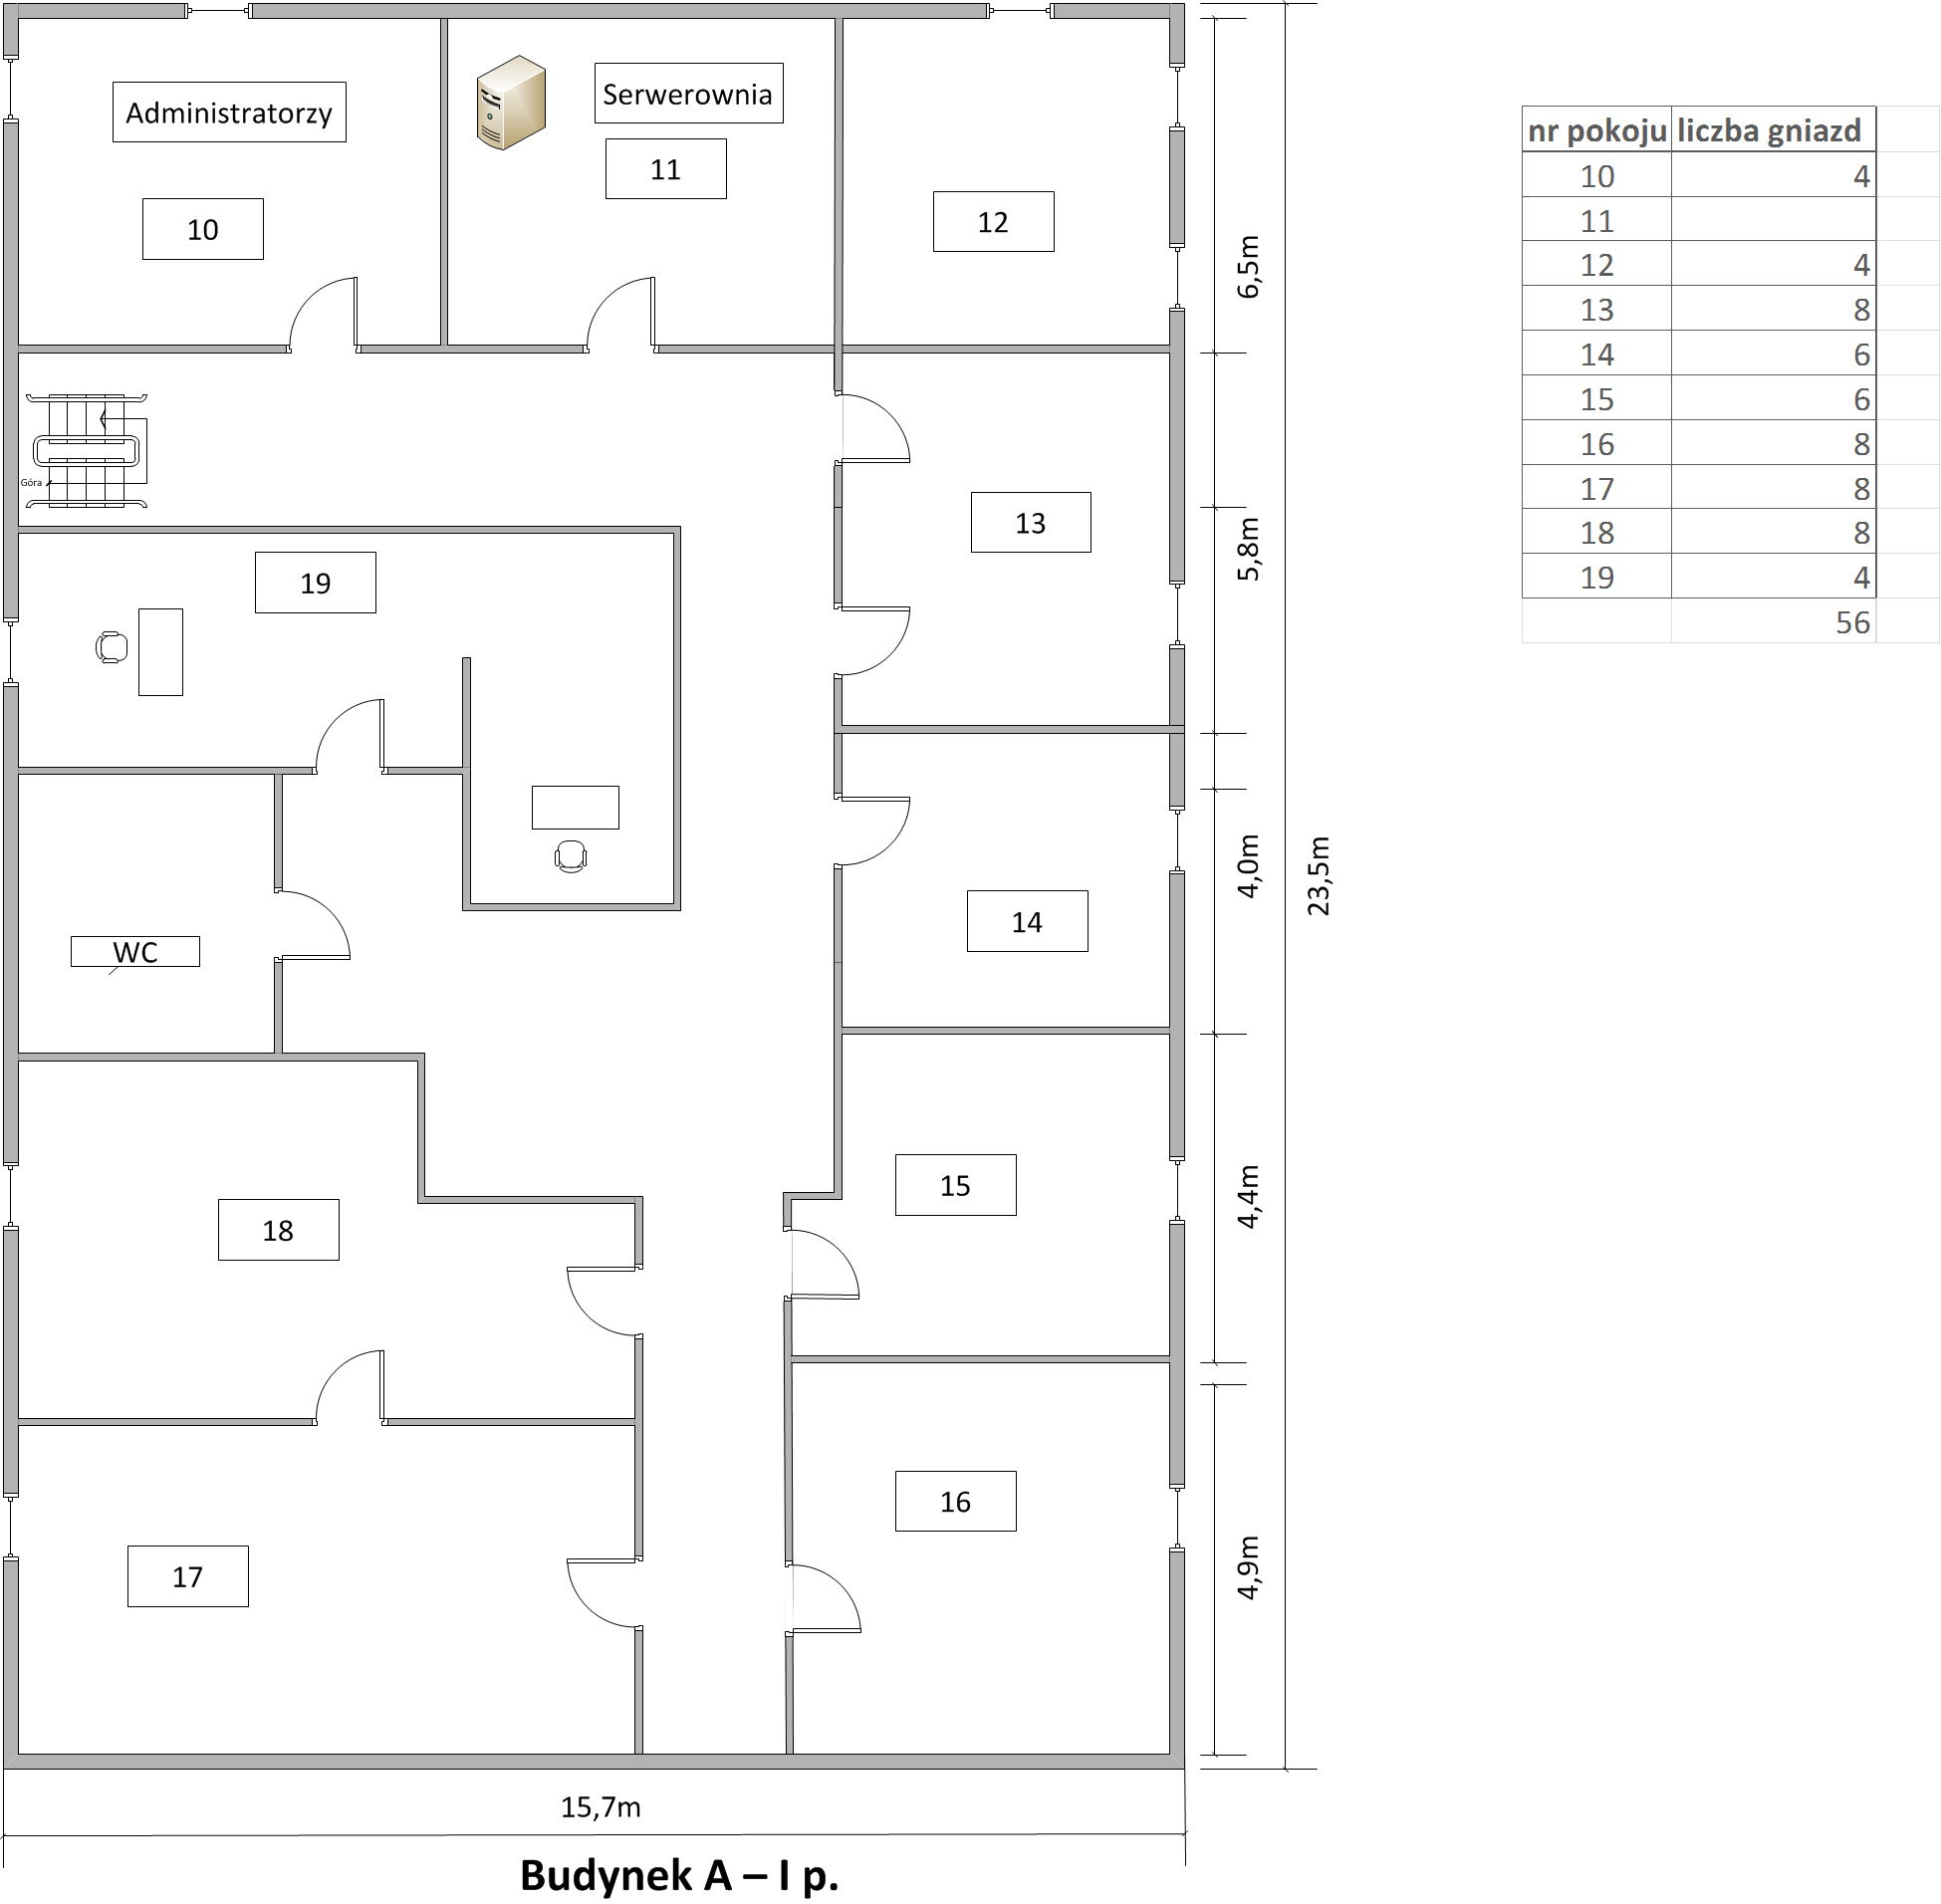
\includegraphics[width=\textwidth]{./obrazki/plany_wew/a1.png}
\end{figure}
\end{comment}
\begin{figure}[H]
  \centering
      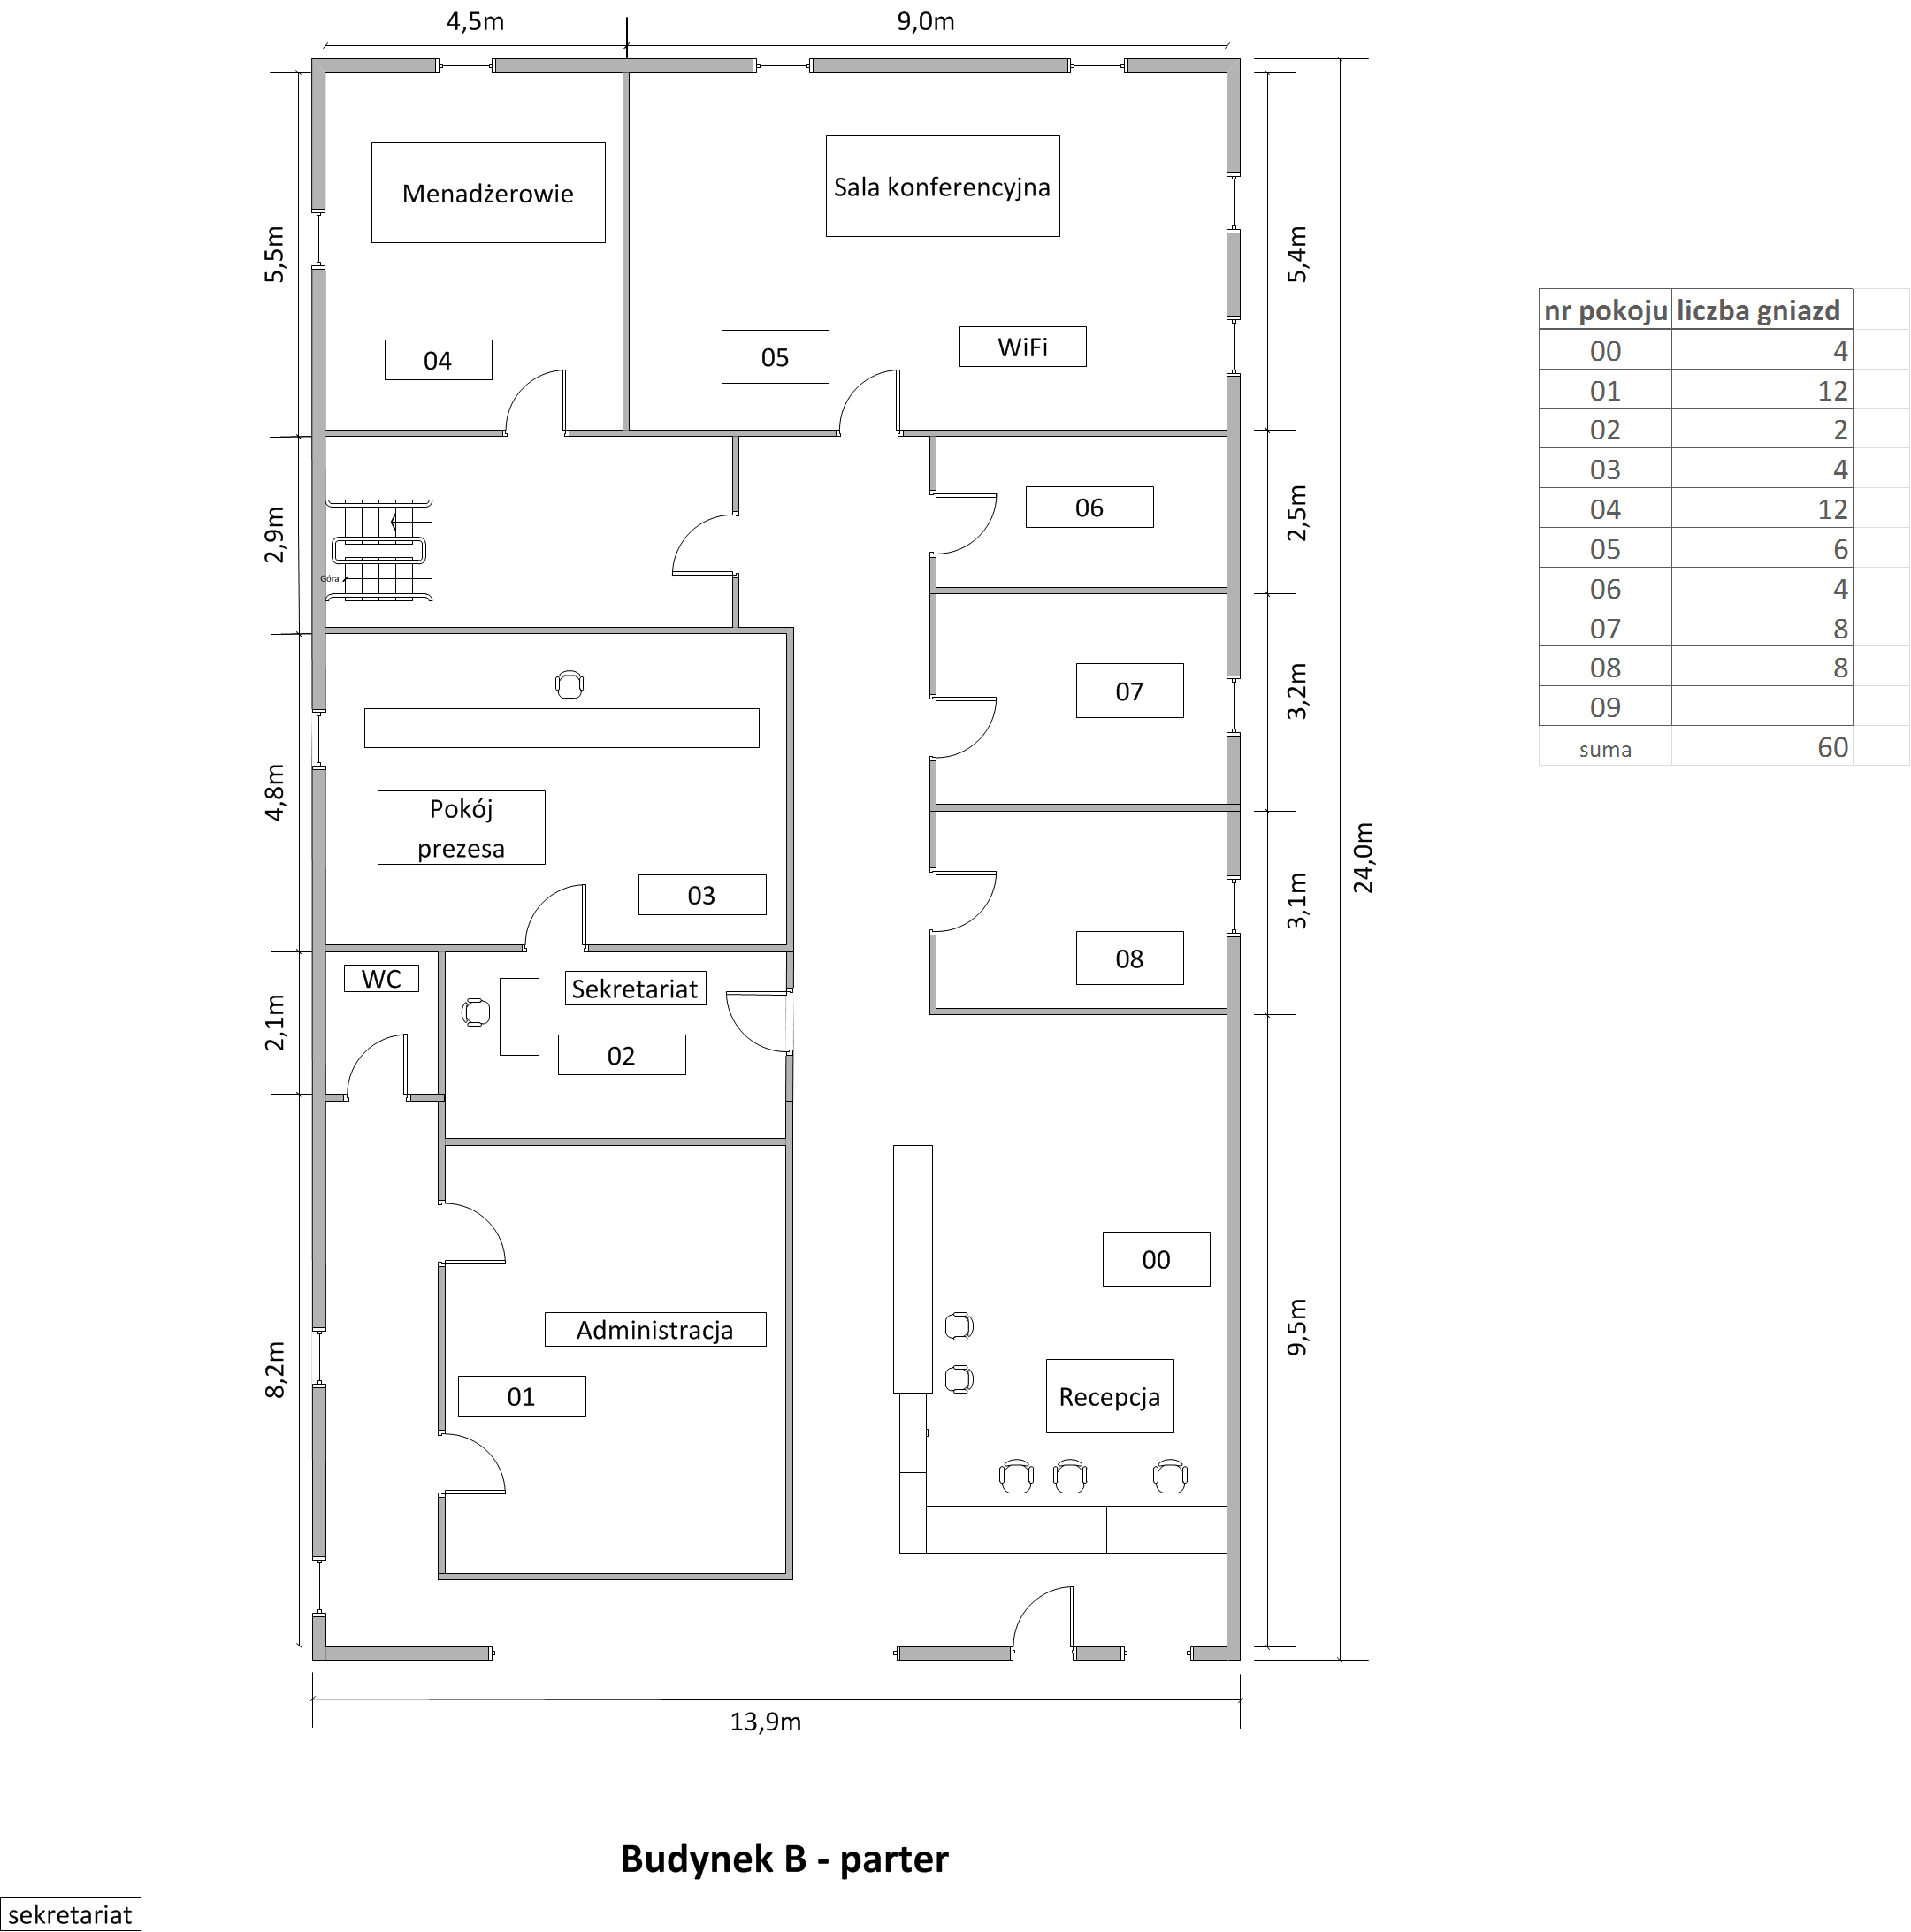
\includegraphics[width=\textwidth]{./obrazki/plany_wew/b0.png}
\end{figure}

\begin{comment}
\begin{figure}[H]
  \centering
      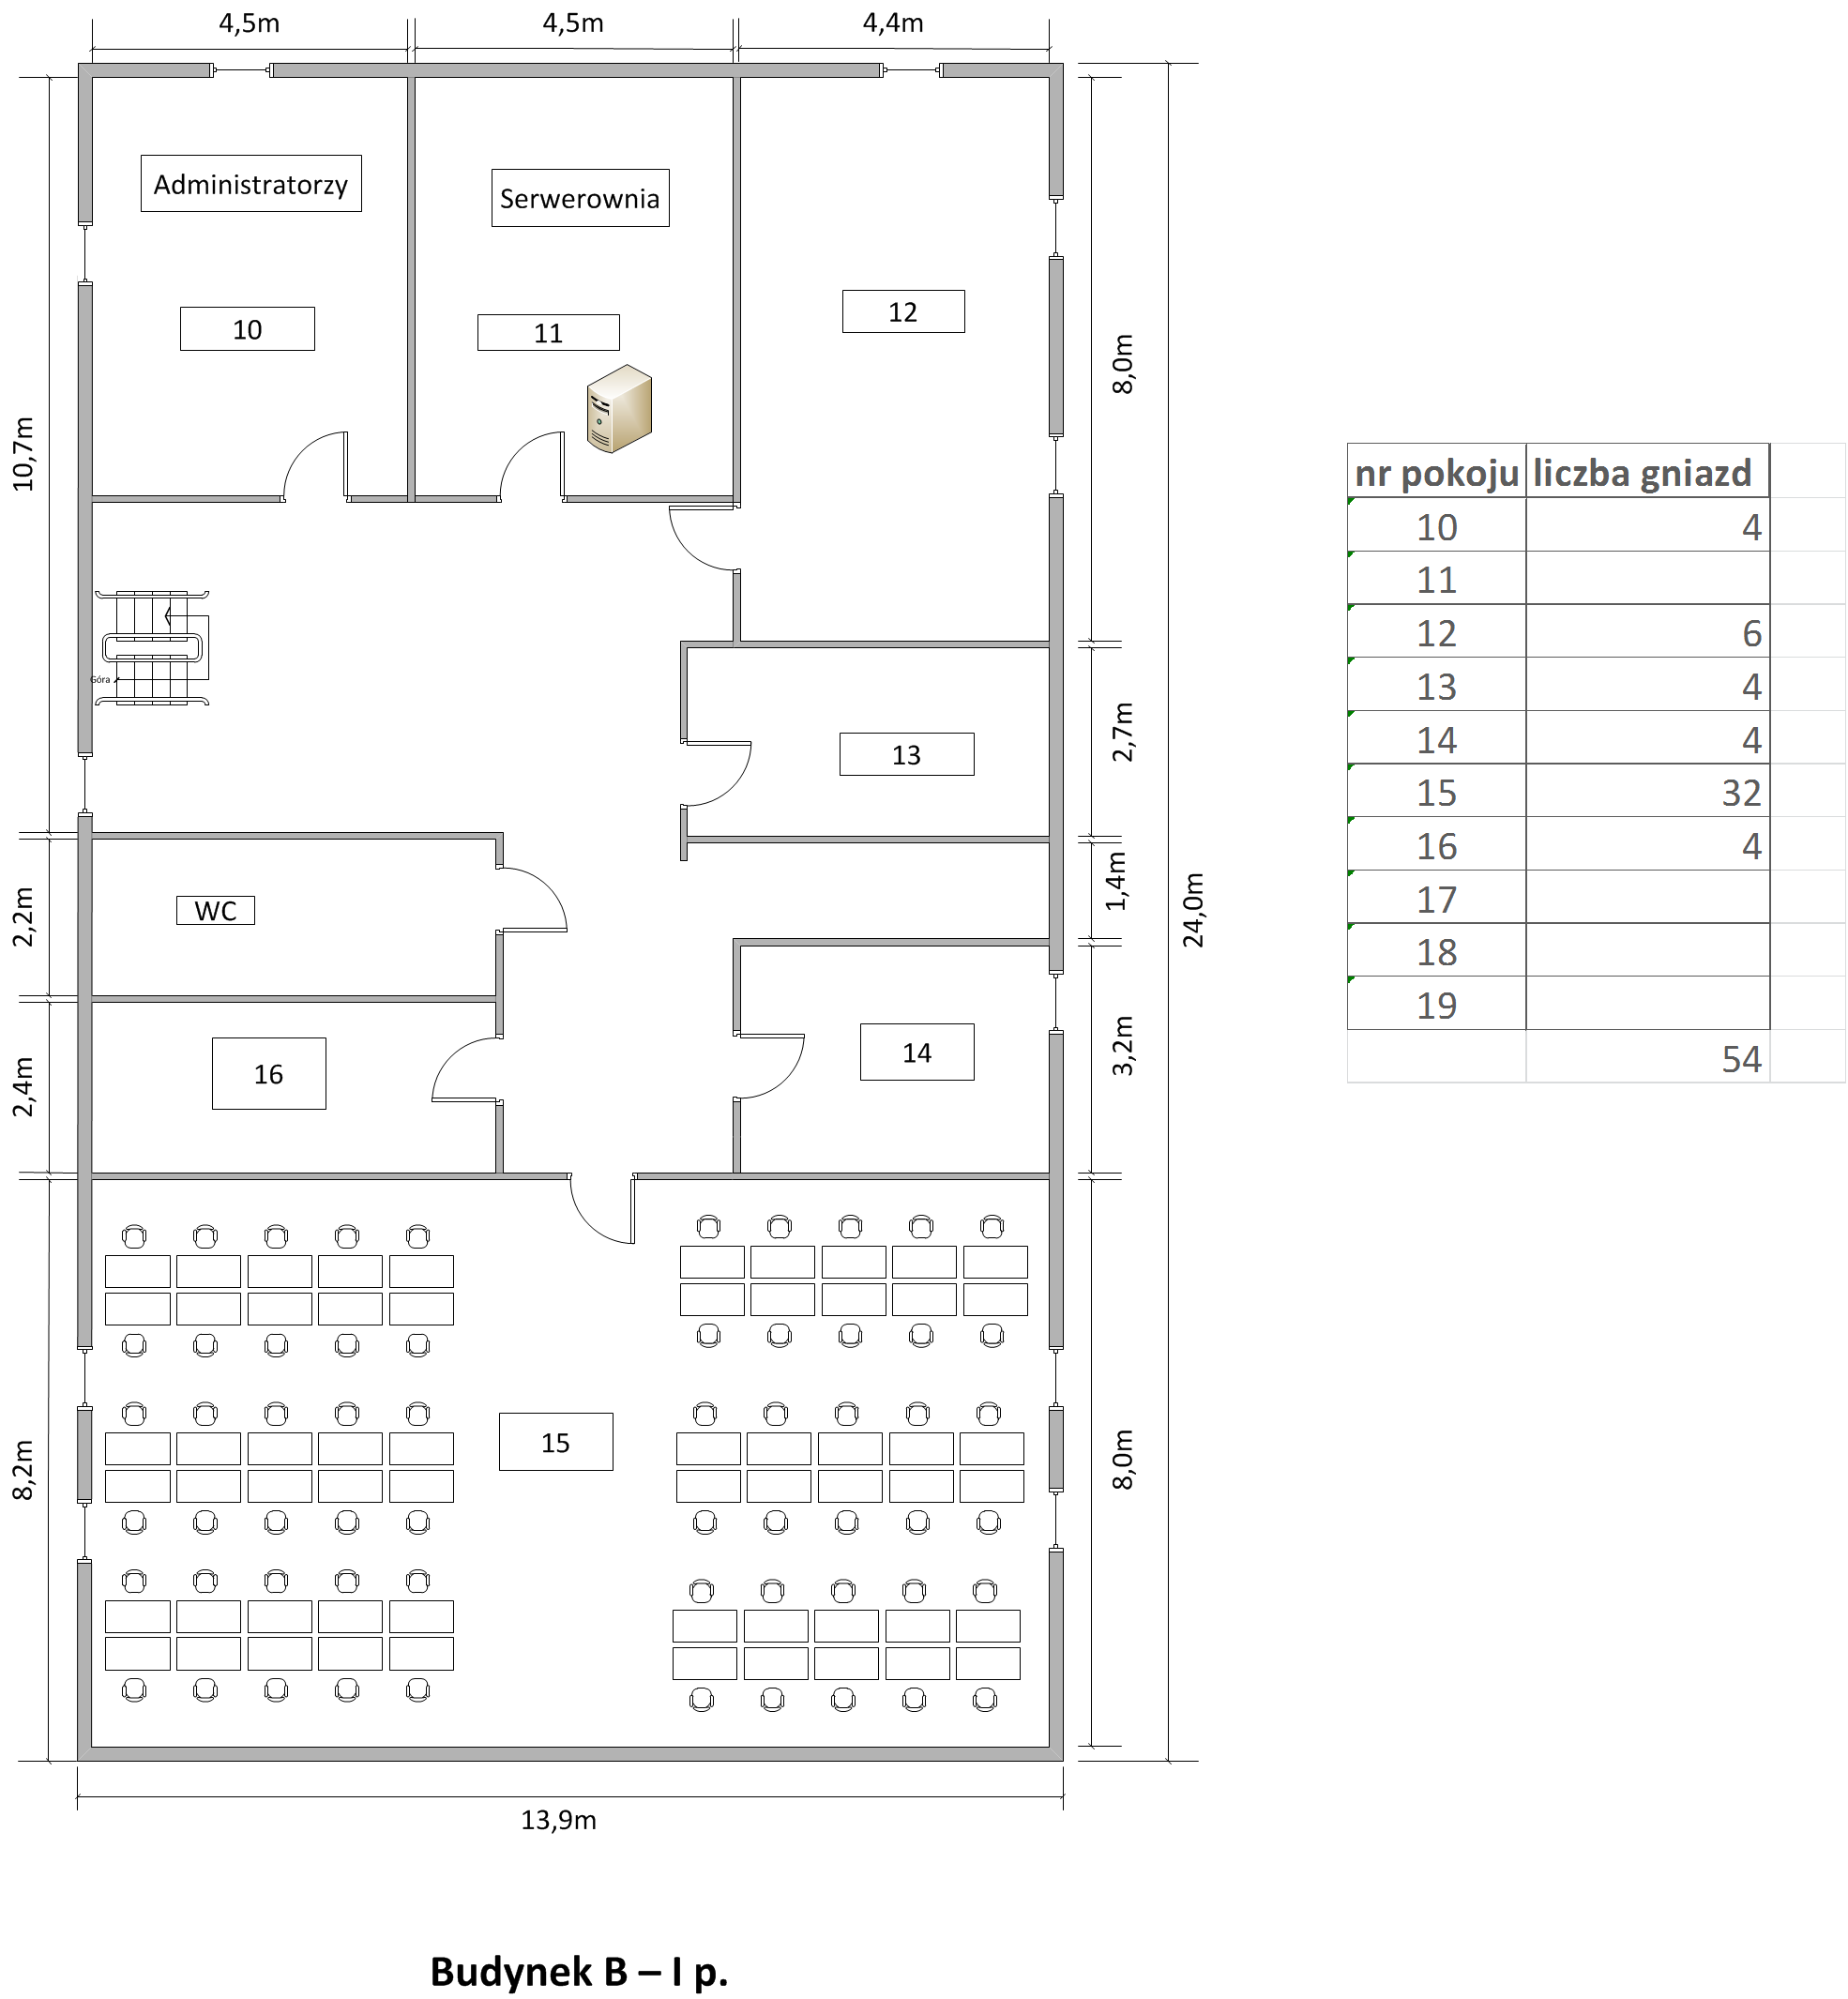
\includegraphics[width=\textwidth]{./obrazki/plany_wew/b1.png}
\end{figure}

\begin{figure}[H]
  \centering
      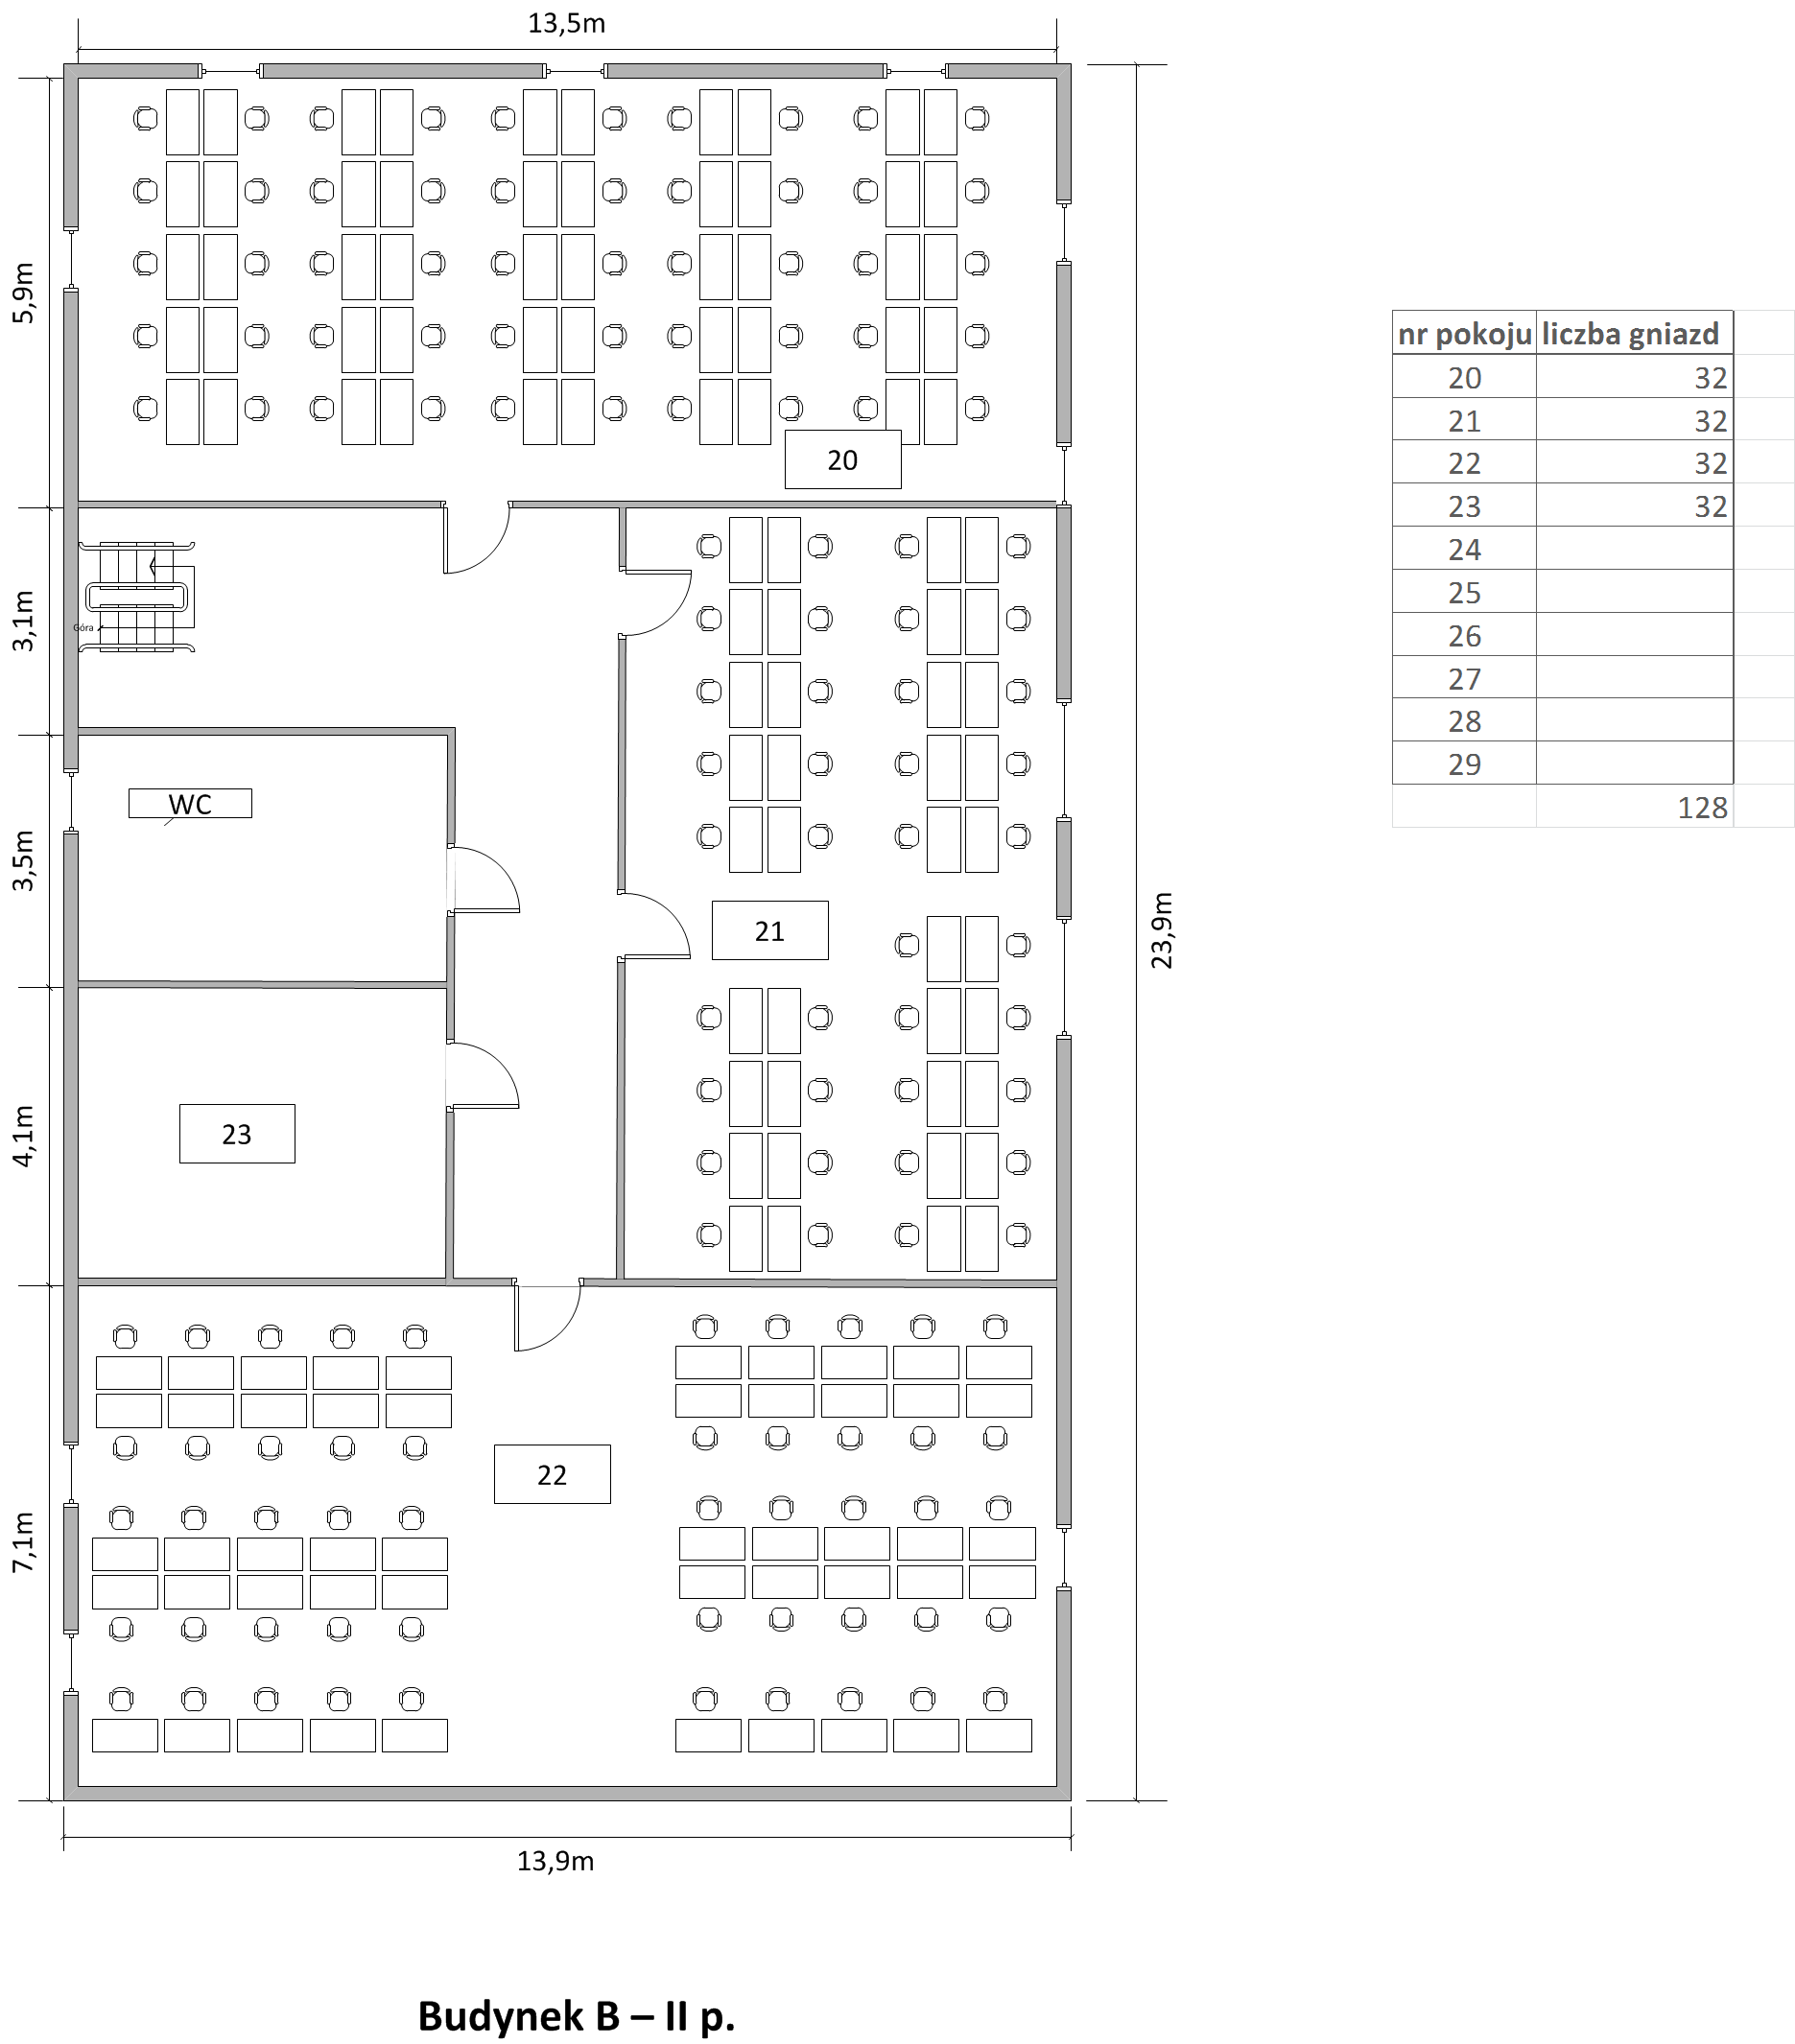
\includegraphics[width=\textwidth]{./obrazki/plany_wew/b2.png}
\end{figure}
\end{comment}


%wzajemne rozmieszczenie budynków
\section{Wzajmne położenie budynków}
\begin{figure}[H]
  \centering
      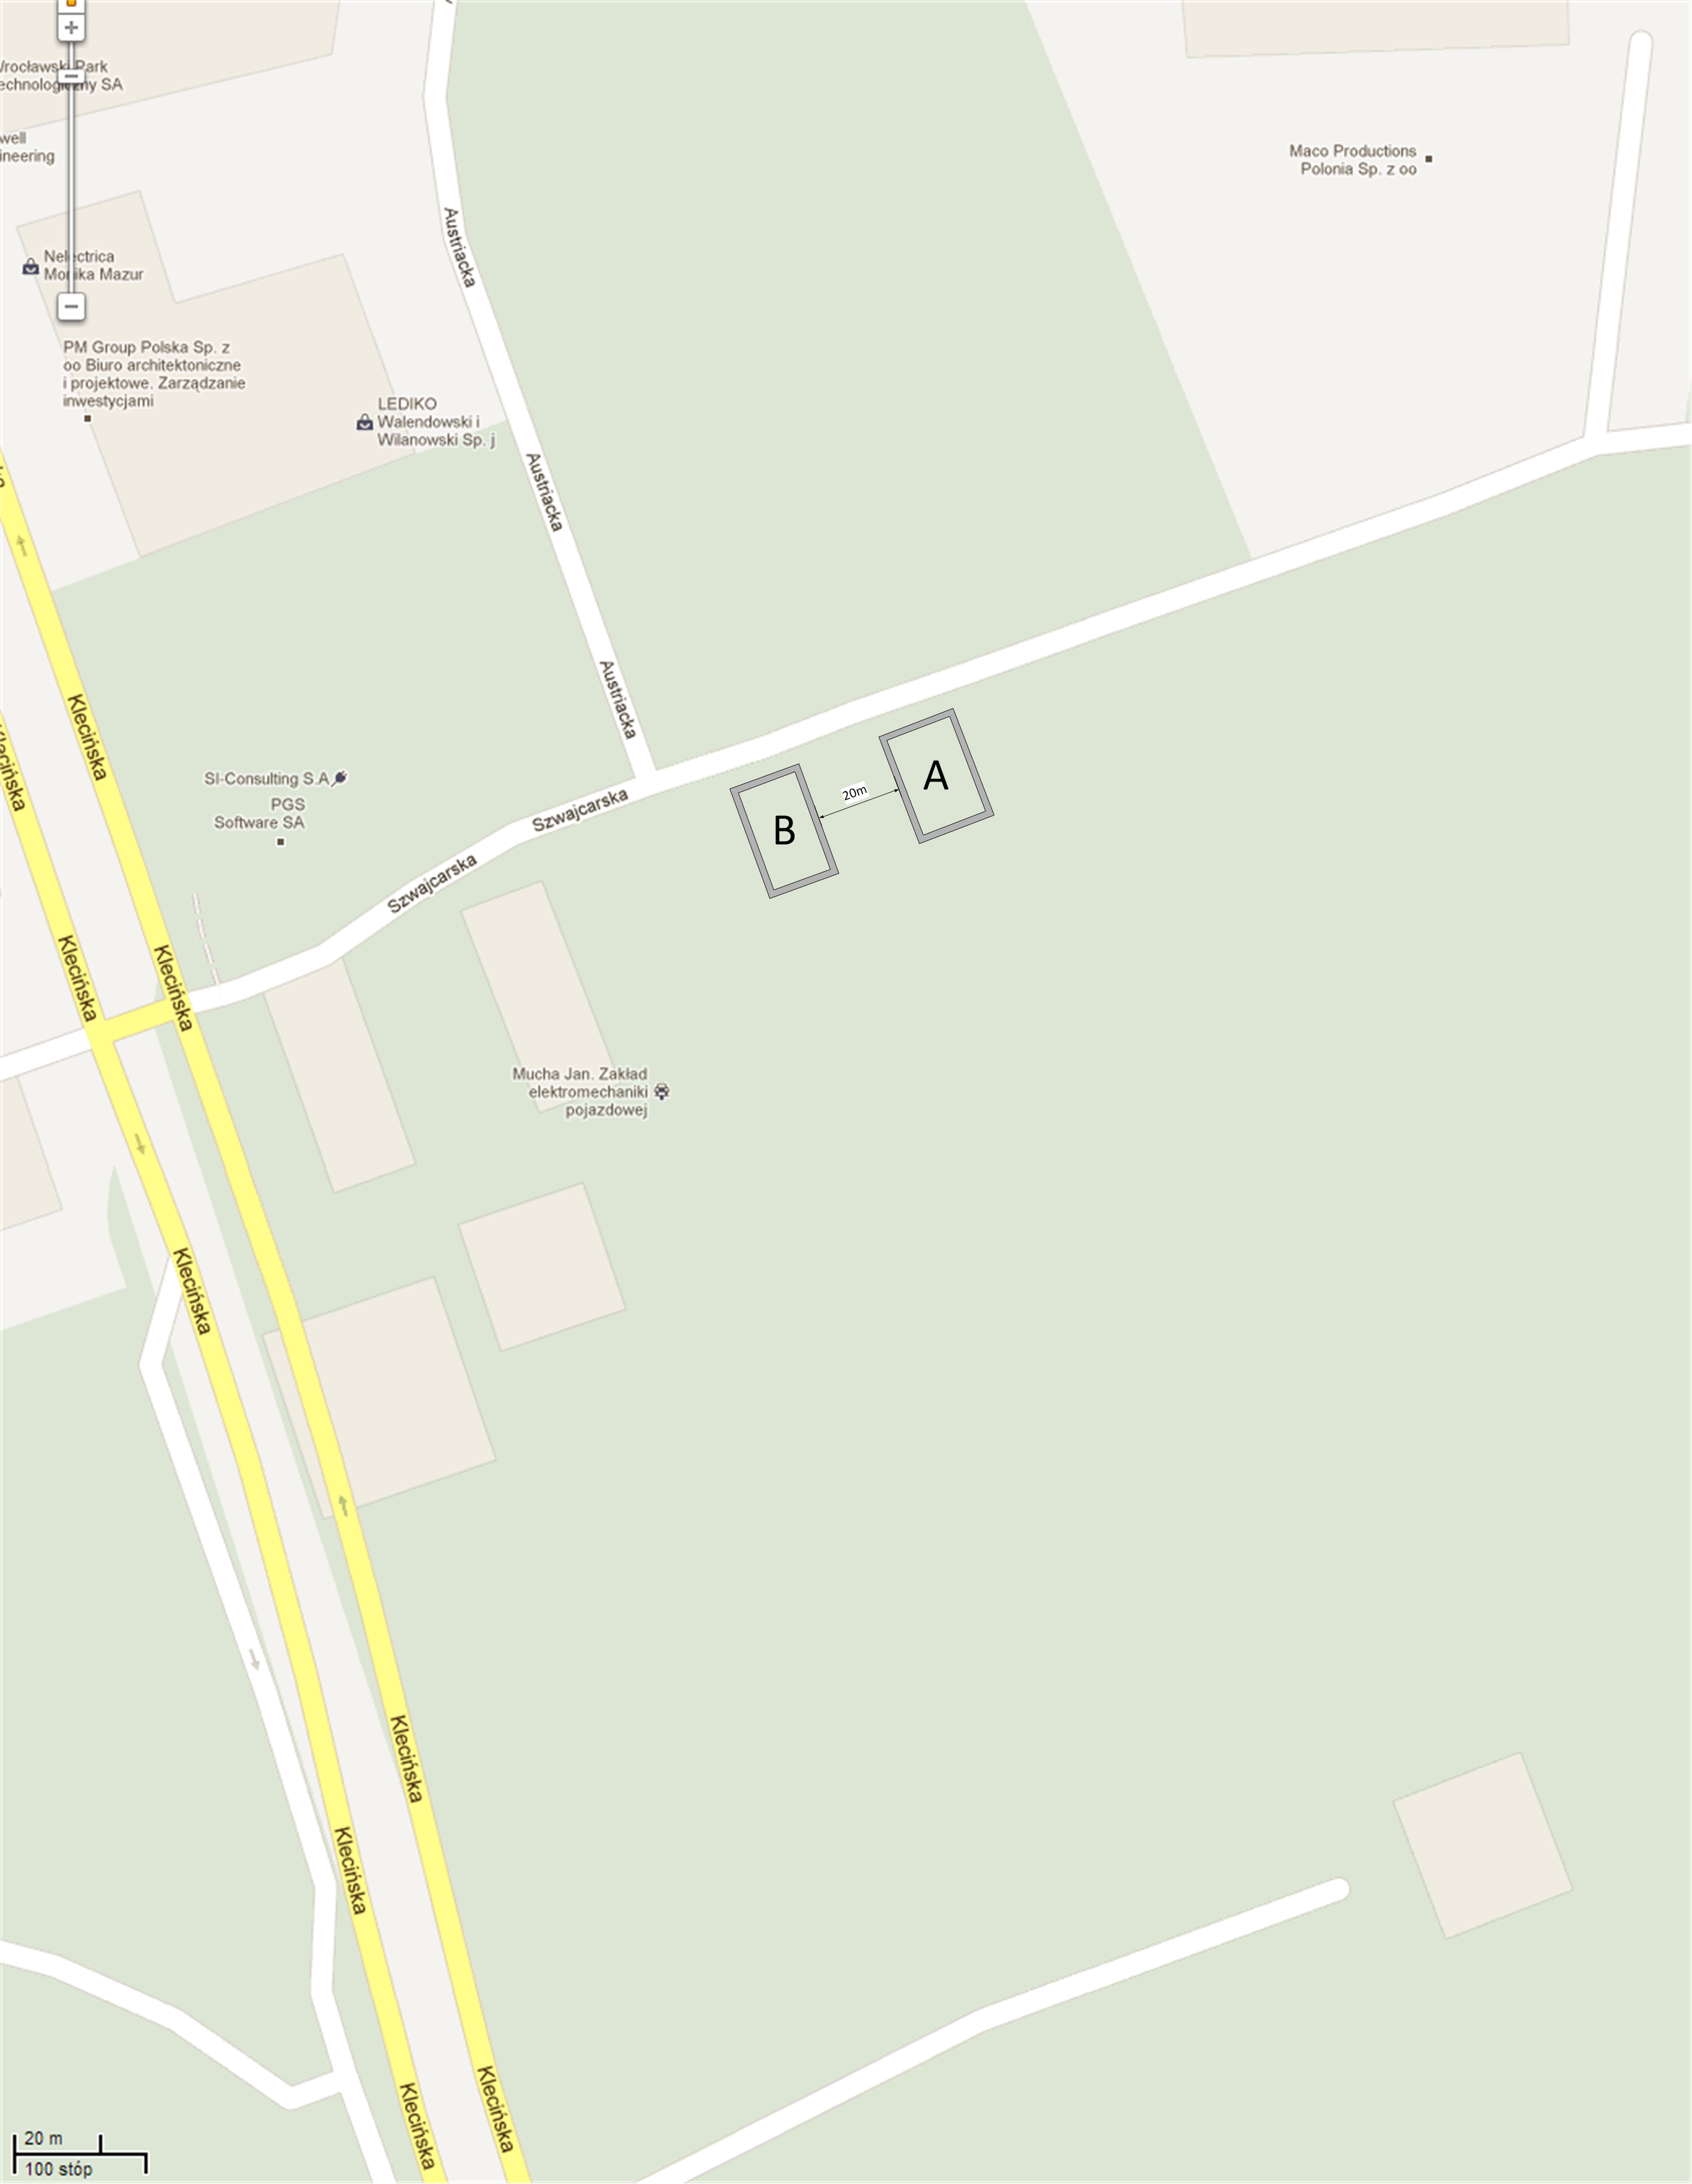
\includegraphics[width=0.5\textwidth]{./obrazki/rzut_terenowy.png}
    \caption{Wzajemne rozmieszczenie budynków na mapie.}
\end{figure}

\begin{figure}[H]
  \centering
      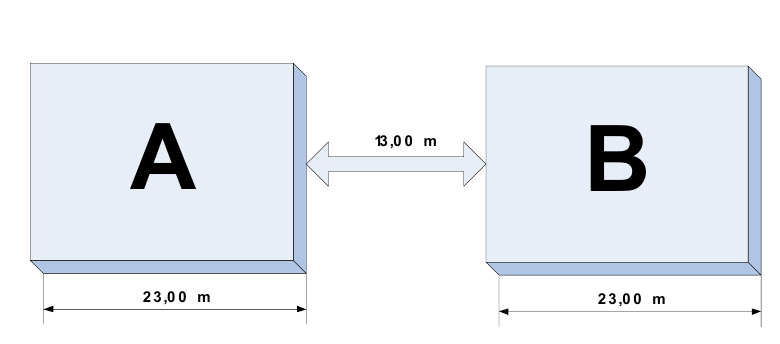
\includegraphics[width=0.8\textwidth]{./obrazki/rozmieszczenie_budynkow.jpeg}
    \caption{Wzajemne rozmieszczenie schemat.}
\end{figure}



\chapter{Analiza potrzeb użytkowników – wymagania zamawiającego}
Na podstawie danych dostarczonych przez firmowego administratora sieci sporządzono analizie ruchu sieciowego jaki wytwarzają
pracownicy w ciągu dnia roboczego. Przedstawiają je tabela 
\ref{tab:analiza dzialy} oraz \ref{tab:analiza podsumowanie}.

\begin{table}[H]

\centering
\caption{Analiza ruchu sieciowego w poszczególnych departamentach.
Tabele reprezentują ilość danych wygenerowanych przez 1 użytkownika danego departametu w ciągu dnia pracy. \label{tab:analiza dzialy}}

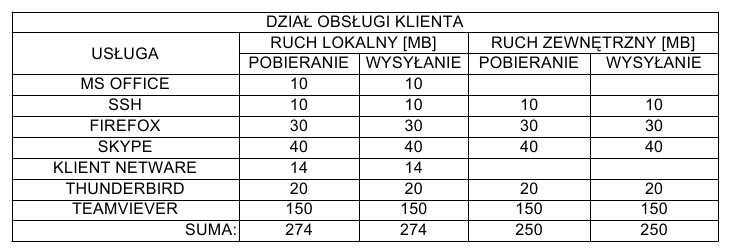
\includegraphics[width=0.5\textwidth]{./obrazki/ruch_tabele/d_ok.png}
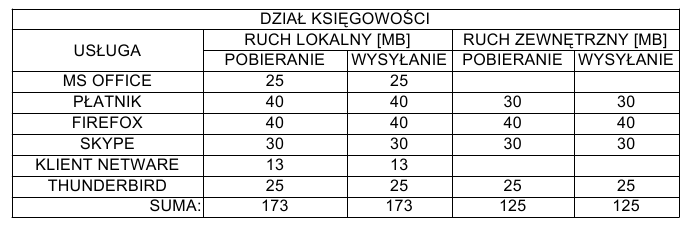
\includegraphics[width=0.5\textwidth]{./obrazki/ruch_tabele/d_k.png}
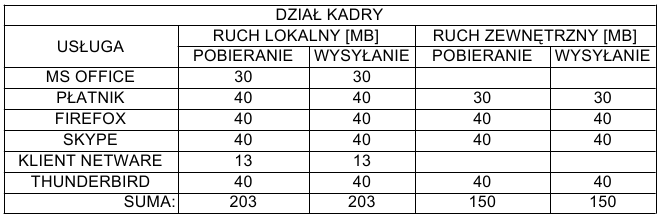
\includegraphics[width=0.5\textwidth]{./obrazki/ruch_tabele/d_kad.png}
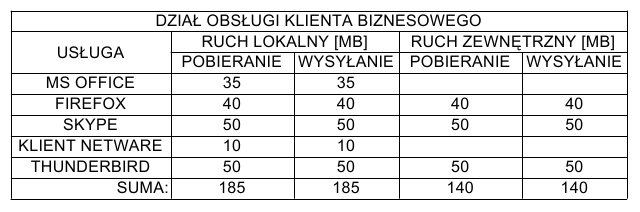
\includegraphics[width=0.5\textwidth]{./obrazki/ruch_tabele/d_b.png}
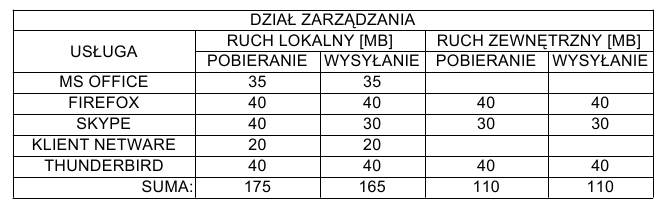
\includegraphics[width=0.5\textwidth]{./obrazki/ruch_tabele/d_m.png}   

\end{table}


\begin{table}[H]

\centering
\caption{Podsumowanie generowanego ruchu. \label{tab:analiza podsumowanie}}

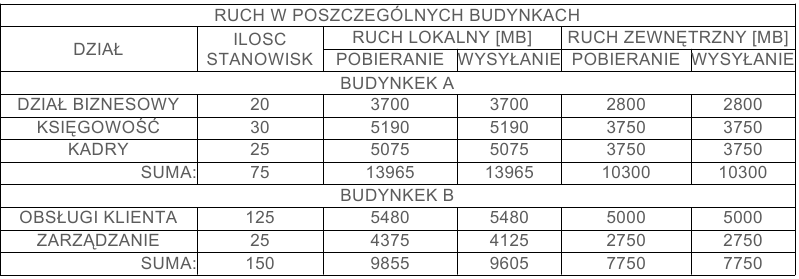
\includegraphics[width=0.6\textwidth]{./obrazki/ruch_tabele/budynki.png}

\hspace{0,5cm}

      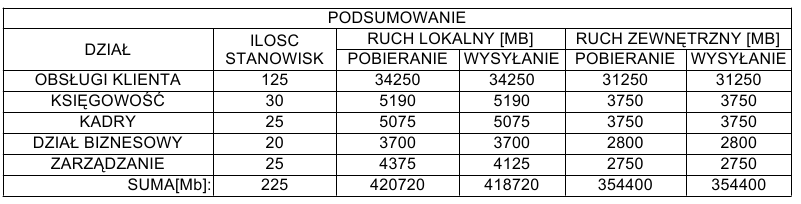
\includegraphics[width=0.5\textwidth]{./obrazki/ruch_tabele/podsumowanie.png}     
 
\end{table}

\paragraph{Punkt abonencki} Liczba punktów abonenckich została przedstawiona w tabeli \ref{table:gniazda na pietro}.Pojedyńczy punkt
abonnencki będzie składał sie z dwóch gniazd RJ45. Jedno przeznaczone dla komputera natomiast drugie dla przyszłych zastosowań.

\begin{table}[H]

\centering
\caption{Planowana liczba punktów abonenckich na piętro zgodnie z wytycznymi klienta. \label{table:gniazda na pietro}}

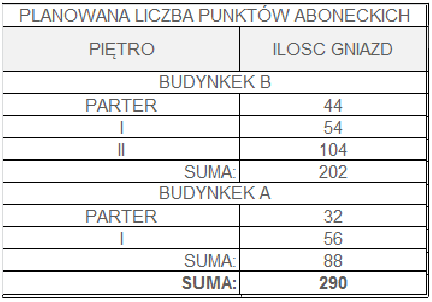
\includegraphics[width=0.4\textwidth]{./obrazki/plany_wew/gniazda_na_pietro.png} 
 
\end{table}

%upieksz jakas ta tabele wyzej

Wszyscy użytkownicy sieci korzystają z następujących programów: klient NetWare,Thunderbird, Firefox, Microsoft Office oraz Skype. Dodatkowo występuje 
oprogramowanie specjalistyczne dla wyszczególnionych działów. Księgowość i kadry pracują dużo na Płatniku natomiast obsługa klienta używa programu
do zdalnego zarządzania innymi komputerami TeamViever oraz ssh.

\paragraph{Plany rozwoju}Firma w najbliższym czasie planuje zakup dodatkowych 5 drukarek sieciowych.Po jednej dodatkowej na każde piętro. Drukarki te mają znajdować się
w ogólnie dostępnym miejscu. Zakup drukarek nie jest częścią tego projektu. W planie sieci ma być jedynie uwzględnione miejsce oraz adresacja dla tych urządzeń.

\paragraph{Poufność danych}ComputerBudy w swojej bazie danych posiada nie tylko dane personalne swoich pracowników ale również klucze kryptograficzne wymagane do połączenia zdalnego
z maszyną klienta. Dane te są newralgiczne dla firmy. W związku z tym trzeba będzie w sieci koniecznie zastosować urządzenie typu firewall.

\paragraph{Serwer www}Serwer na którym jest umieszczona strona firmy do poprawnego obsługiwania zapytań potrzebuje łącze o przepustowości 0,5 Mb/s do pobierania oraz
1 Mb/s do wysyłania.  Wartości te będą uwzględnione dla wymagań dotyczących łącza internetowego. Dostęp z zewnątrz do serwera ma być realizowany przy pomocy mechanizmu port forwarding.

\paragraph{Backup}Codziennie od godziny 24:00 do 6:00 rano wykonywany jest backup bazy danych klientów. Aby został poprawnie wykonany wymagana jest przepustowość 
na poziomie 3 Mb/s. Ponieważ czynność ta wykonywana jest w nocy wymaganie to będzie na pewno spełnione gdyż pracownicy nie będą generować ruchu
sieciowego.

\paragraph{Sieć wifi}Klient wyraził zapotrzebowanie na instalację sieci wifi dla działu obsługującego przedsiębiorców. W sali konferencyjnej często dochodzi  
do spotkań z klientami oraz małych narad zarządu. Wygodny dostęp dla internetu na pewno byłby czynnikiem ułatwiającym wszelkie negocjacje.
Niestety nie można przewidzieć zapotrzebowania na pasmo dla tego elementu sieci ponieważ nie wiadomo jaki program zechce uruchomić użytkownik.
Nie jest to obciążenie ciągłe sieci więc odpowiedni zapas przepustowości powinien rozwiązać ten problem.

Na podstawie zebranych danych można postawić wymagania dotyczące przepustowości sieci lokalnej oraz łącza z internetowego. Tabela \ref{tab:parametry_loncza}
prezentuje wymagania minimalne oraz zalecane. Wymagania minimalne zawierają wartości parametrów niezbędnych do poprawnego działania sieci. 
Niestety gdyby ich użyć mogłyby wystąpić problemy z jakością usług gdyby jakiś program przeciążył sieć. Aby tego uniknąć należy użyć wartości
zalecanych, które stanowią trzykrotność wartości minimalnej. Z takim zapasem przepustowości sieć będzie odporna na większość przeciążeń.


\begin{table}[H]
\caption{Przepustowości łącza internetowego. }
\label{tab:parametry_loncza}
 \centering
      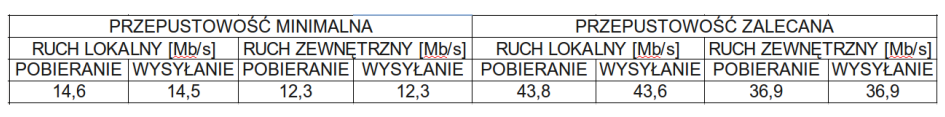
\includegraphics[width=0.8\textwidth]{./obrazki/ruch_tabele/loncze.png}
\end{table}


\chapter{Założenia projektowe}

Na podstawie analizy potrzeb ComputerBudy, proponujemy
następujące rozwiązania:

\begin{itemize}

\item{technologia Gigabit Ethernet wykorzystana w okablowaniu pionowym}

\item{technologia Fast Ethernet wykorzystana w okablowaniu poziomym}

\item{symetryczne łącze z dostępem do Internetu o przepustowości 40 Mb/s}

\item{strukturę sieci oddzielającą serwery lokalne od zewnętrznych:
 \begin{itemize}
\item serwer WWW,
\item serwer bazy danych,
\end{itemize}}

\item {zabezpieczenie zasilania serwerów urządzeniami UPS}

\item {użycie kabla UTP z kategorii 6,}

\item {urządzenia kompatybilne z IPv6 (router’y, switch’e, serwery),}

\item {urządzenia obsługujące technologię QoS}

\item{technologię VLAN w celu odseparowania jednostek organizacyjnych firmy}

\item{bezprzewodowy dostęp do sieci w dziale obługi klienta biznesowego w technologii WiFi
802.11n na częstotliwości 2,4Ghz}

\item{bezpieczeństwo sieci zapewnione firewall’em}

\item{dodatkowo ochrona realizowana przez specyfikę technologii VLAN,}

\item{skalowalność dzięki zhierarchizowanemu podziałowi warstw.}

\end{itemize}


\chapter{Projekt sieci}
\section{Projekt logiczny sieci wraz z opisem koncepcji rozwiązania}
\subsection{Ogólna koncepcja}

Cała sieć zostanie podzielona na dwie strefy. Pierwsza zdemilitaryzowana w której będą znajdować się serwery WWW oraz bazy danych. 
Zostaną one podłączone do przełącznika warstwy 2 za pomocą pomocą łączy o przepustowości 100Mb/s. Przełącznik z ruterem zostanie połączony 
przy pomocy łącza o prędkości 1Gb/s. Druga będzie to wewnętrzna prywatna sieć firmy z komputerami pracowników oraz wewnętrzna sieć wifi firmy. 
Strefa prywatna dla osiągnięcia większego poziomu bezpieczeństwa zostanie podzielona na wirtualne podsieci połączone za pomocą przełączników w warstwie 3. Każdy odział firmy
oraz sieć wifi będzie stanowić osobną podsieć wirtualną. Każde piętro będzie posiadło swój przełącznik w warstwie 2 do którego będą
doprowadzone połączenia z hostów znajdujących się na danym piętrze o przepustowości 100Mb/s.
Punkt dostępu wifi zostanie  podpięty do normalnego switcha również łączem o przepustowości 100Mb/s. Wszystkie switche opreujące
w warstwie 2 będą zbudowane przy pomocy funkcji stackable. W każdym budynku będzie znajdował 
się 1 switch obsługujący wirtualne sieci. Switche obsługujące poszczególne piętra oraz ruter będzie z nimi połączony za pomocą łączy o przepustowości 1Gb/s.
Switch warstwy 3 z budynku A będzie podłczony do odpowiadającego mu swicha w budynku B. Właśnie to połączenie będzie przebiegać pomiędzy budynkami. Oczywiście
będzie ono miało przepustowość 1Gb/s. Switch warstwy 3 w budynku B będzie podłączony do rutera również takim złączem. 
Połączenie do sieci internet zostanie oddzielone za pomocą firewala dla zwiększenia bezpieczeństwa.

\subsection{Toplogia sieci}
\begin{figure}[H]
  \centering
      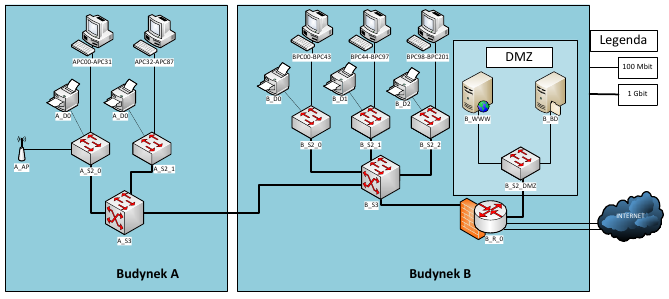
\includegraphics[width=0.9\textwidth]{./obrazki/topo_log.png}
  \caption{Topologia logiczna sieci.}
\end{figure}

\begin{table}[H]
\caption{Proponowane modele urządzeń.\label{table:proponowane_urzadzenia}}
 \centering
      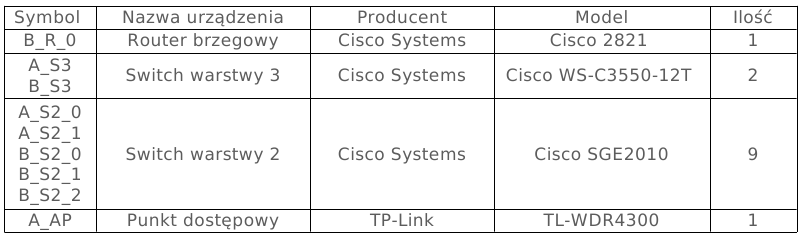
\includegraphics[width=0.8\textwidth]{./obrazki/spis_przyrzadow.png}
\end{table}

\subsection{Projekt podziału na VLAN}
\begin{figure}[H]
  \centering
      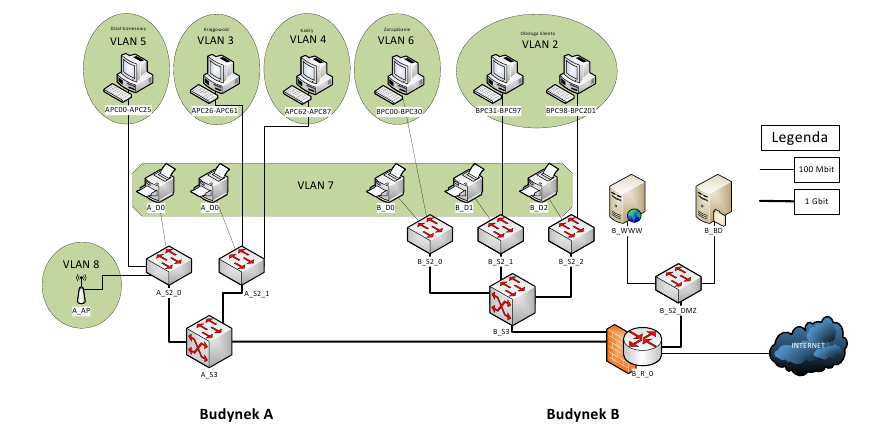
\includegraphics[width=0.9\textwidth]{./obrazki/topo_vlan.png}
  \caption{Projekt podziału na VLAN.}
\end{figure}

\section{Konfiguracja adresacji IP}
\subsection{Podział na VLAN}
Jak już wcześniej było wspomniane tworzona przez nas sieć ma zapewniać bezpieczeństwo oraz łatwą adaptacje sieci do nowych warunków.
Jedną z metod jakie wybraliśmy do uzyskania tego jest VLAN. Uzyskamy dzięki tej technologi separacja pomiędzy poszczególnymi
sekcjami firmy. Ponadto umożliwi to łatwe zarządzanie ruchem przez administratora. Podział sieci firmowej za pomocą VLAN przedstawia tabela \ref{table:konf_vlan}.
% u mnie w pdf'ie tu dwa pytajniki są ??

\begin{table}[H]
\caption{Podział sieci firmowej na poszczególne VLANY}
\label{table:konf_vlan}
 \centering
      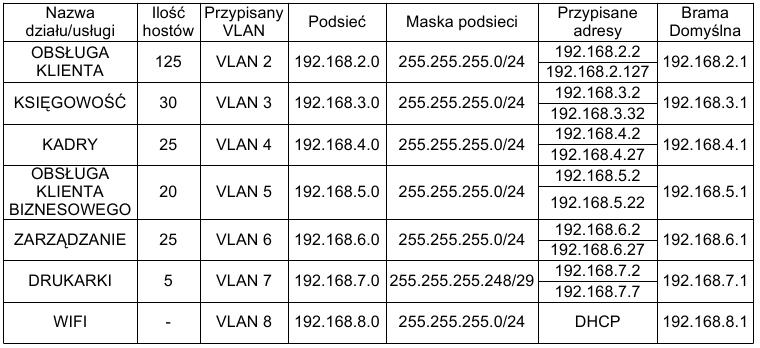
\includegraphics[width=0.8\textwidth]{./obrazki/ip/ip_vlan.png}
\end{table}

Podczas adresacji w tabeli \ref{table:konf_vlan} celowo został ominięty VLAN 1 aby była możliwa współpraca z urządzeniami z firmy CISCO.
Urządzenia tej firmy  obsługujące technologię VLAN, domyślnie tworzą sieć VLAN 1, która odpowiada za zarządzanie utworzoną siecią i za
 przekazywanie komunikatów w różnych protokołach.

\subsection{Adresacja w strefie DMZ}
Adresy w strefie DMZ zostały szczegółowo określone w tabeli \ref{table:konf_dmz} aby administrator sieci mógł dokładnie kontrolować ruch płynący na poszczególne serwery.
\begin{table}[H]
\caption{Adresy przypisane do poszczególnych serwerów w strefie DMZ.}
\label{table:konf_dmz}
 \centering
      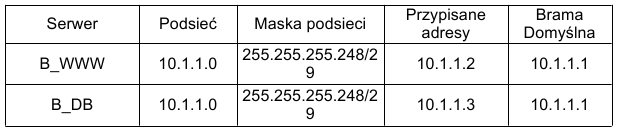
\includegraphics[width=0.8\textwidth]{./obrazki/ip/ip_dmz.png}
\end{table}

\subsection{Adresacja interfejsów }
Prawidłowa konfiguracja interfejsów fizycznych jak i wirtualnych ma kluczowe znaczenie dla poprawności działania sieci. Została ona szczegółowa wypisana
dla poszczególnych interfejsów w poniższych tabelach. Użyto oznaczeń charakterystycznych dla firmy CISCO ponieważ są ogólnie znane i dość 
intuicyjne.

\begin{table}[H]
\caption{Adresy ip przypisane do interfejsów dla rutera.}
 \centering
      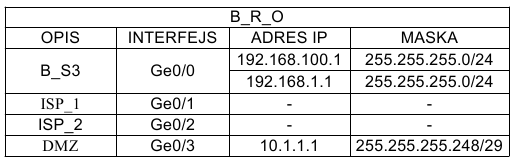
\includegraphics[width=0.6\textwidth]{./obrazki/ip/br0.png}
\end{table}

\begin{table}[H]
\caption{Adresy ip przypisane do interfejsów switcha warstwy 3 w budynku B.}
 \centering
      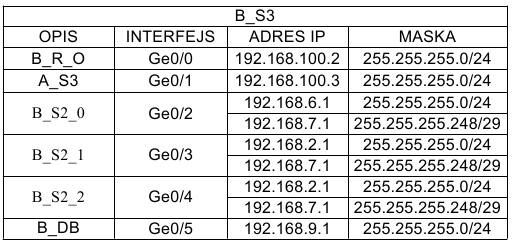
\includegraphics[width=0.6\textwidth]{./obrazki/ip/bs3.png}
\end{table}

\begin{table}[H]
\caption{Adresy ip przypisane do interfejsów switcha warstwy 3 w budynku A.}
 \centering
      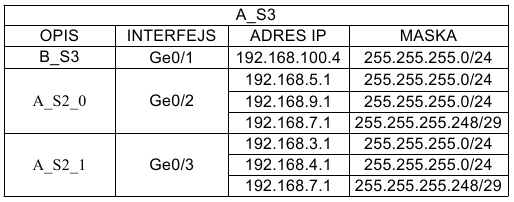
\includegraphics[width=0.6\textwidth]{./obrazki/ip/as3.png}
\end{table}

\section{Projekt okablowania}

\subsection{Plan rozmieszczenia okablowania}

\begin{figure}[H]
  \centering
      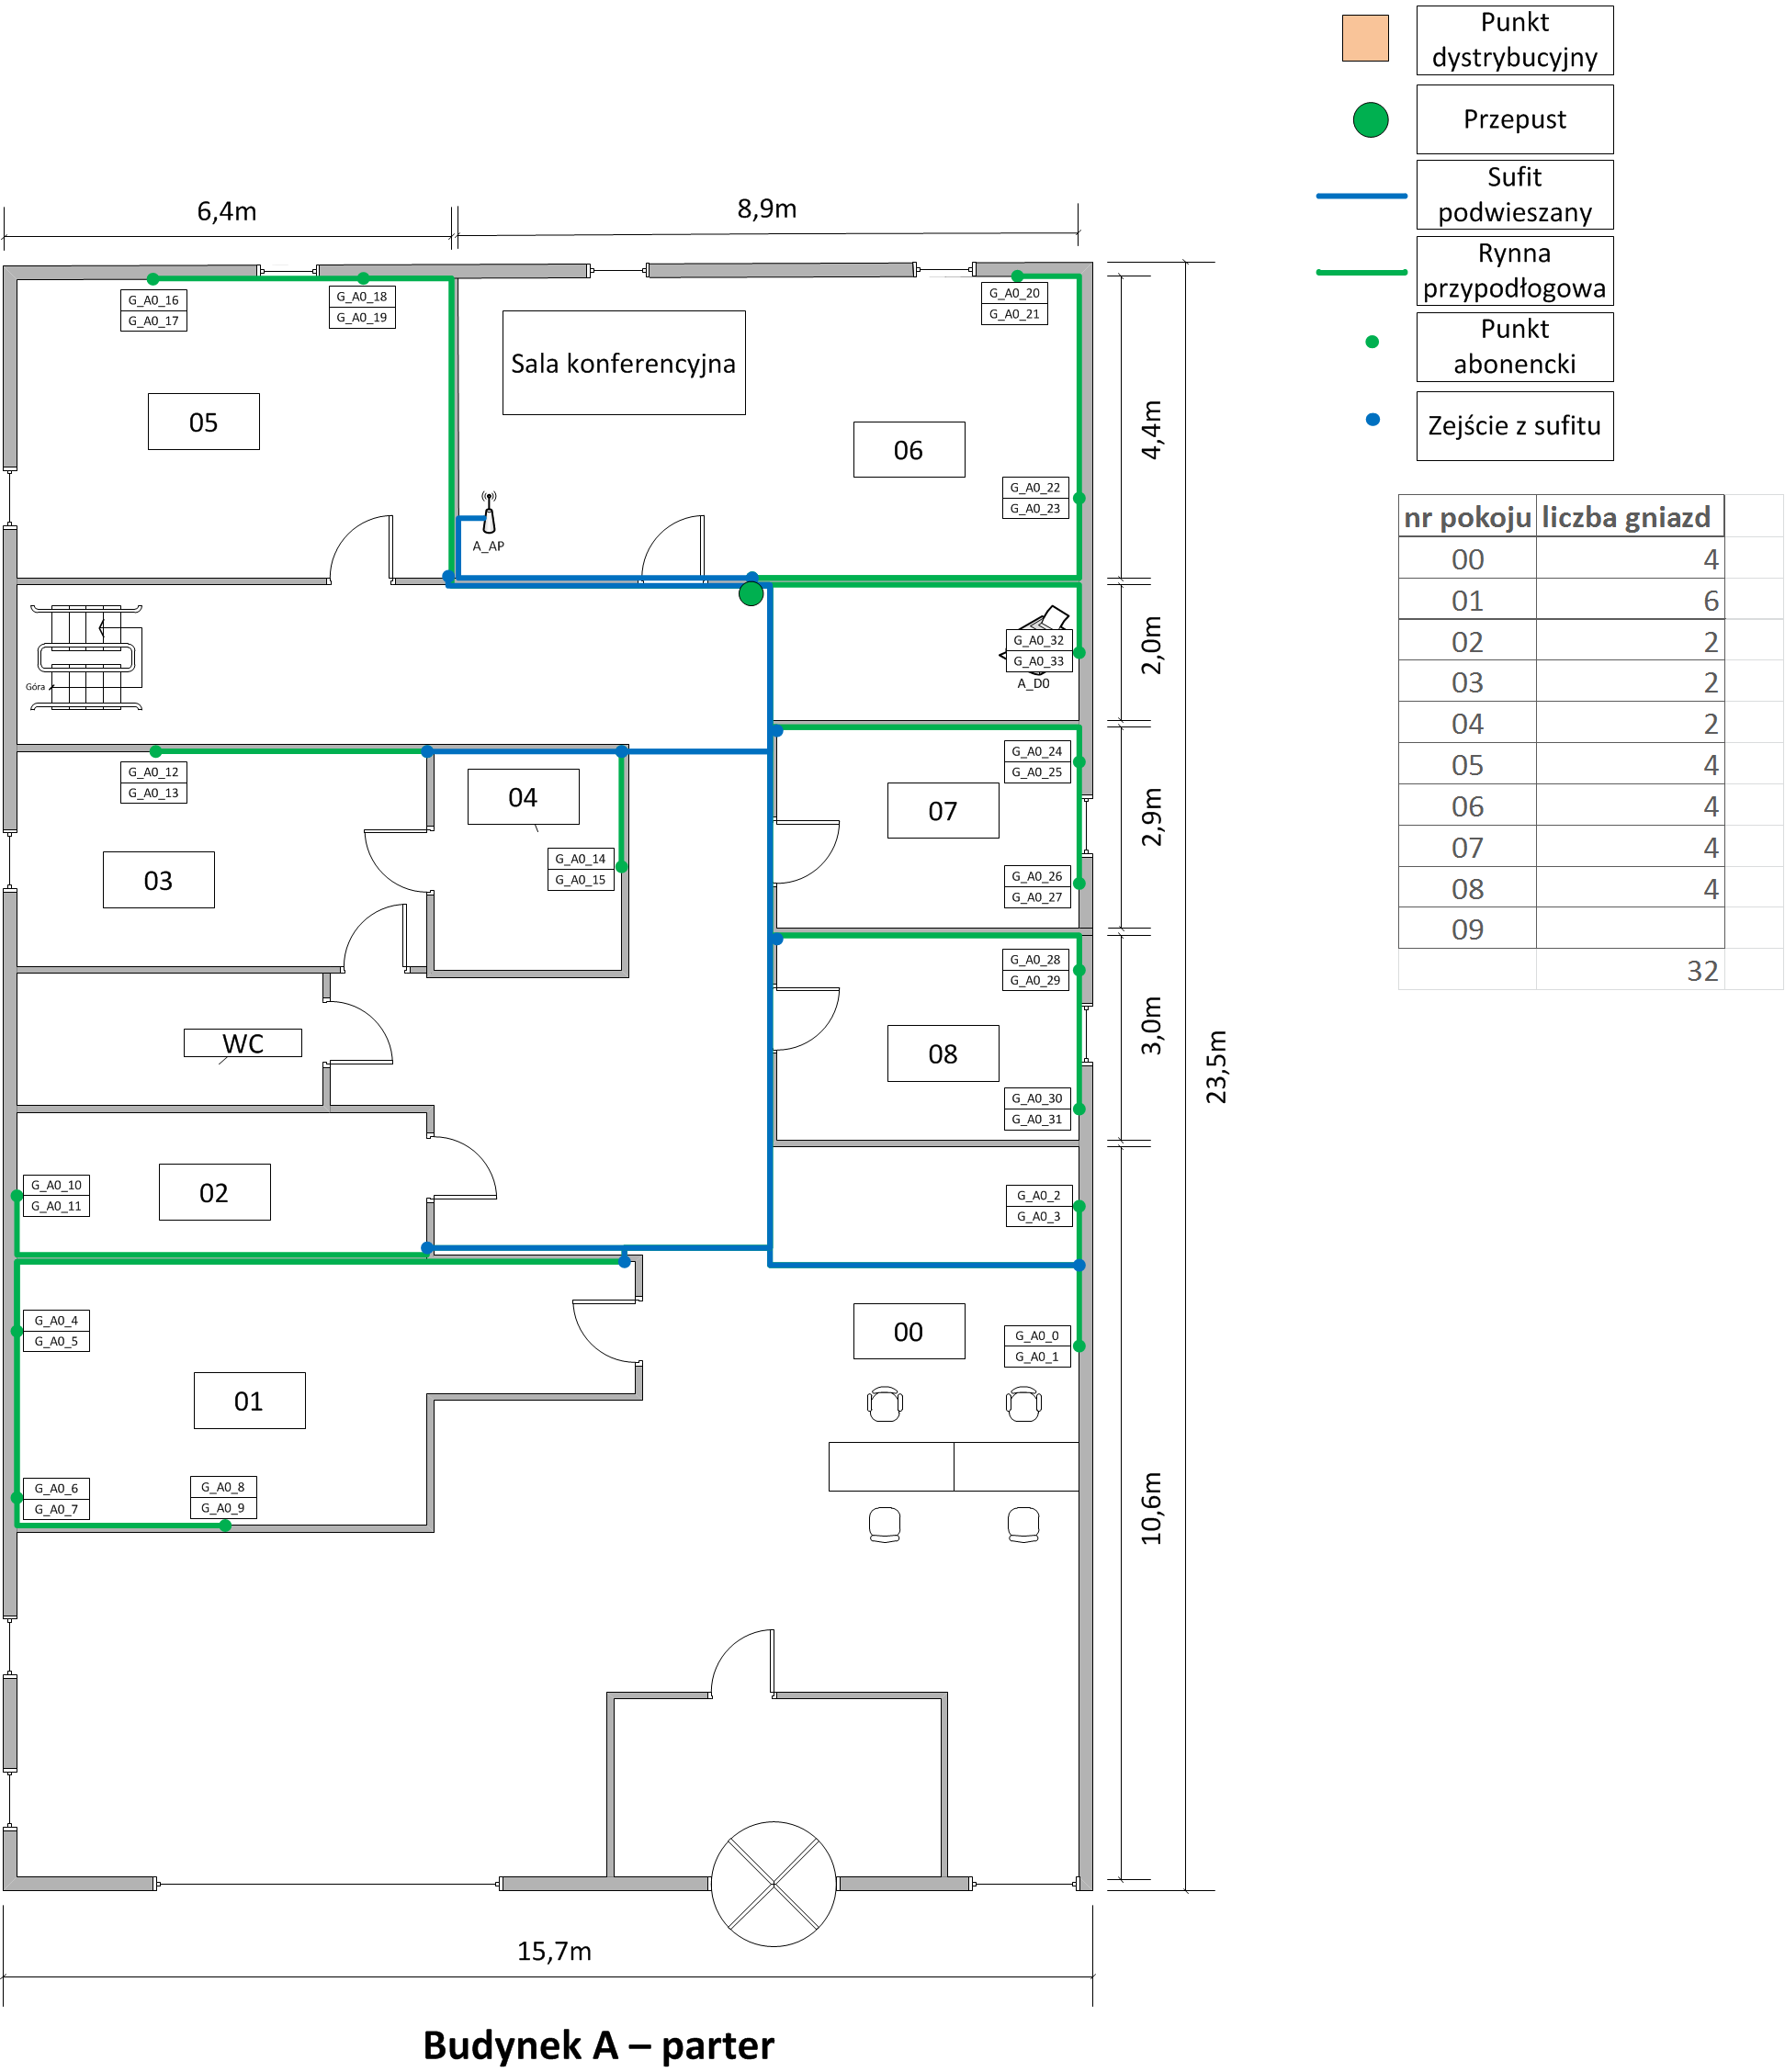
\includegraphics[width=\textwidth]{./obrazki/kable/a0.png}
  \caption{Projekt rozmieszczenia okablowania na parterze w budynku a.}
\end{figure}

\begin{figure}[H]
  \centering
      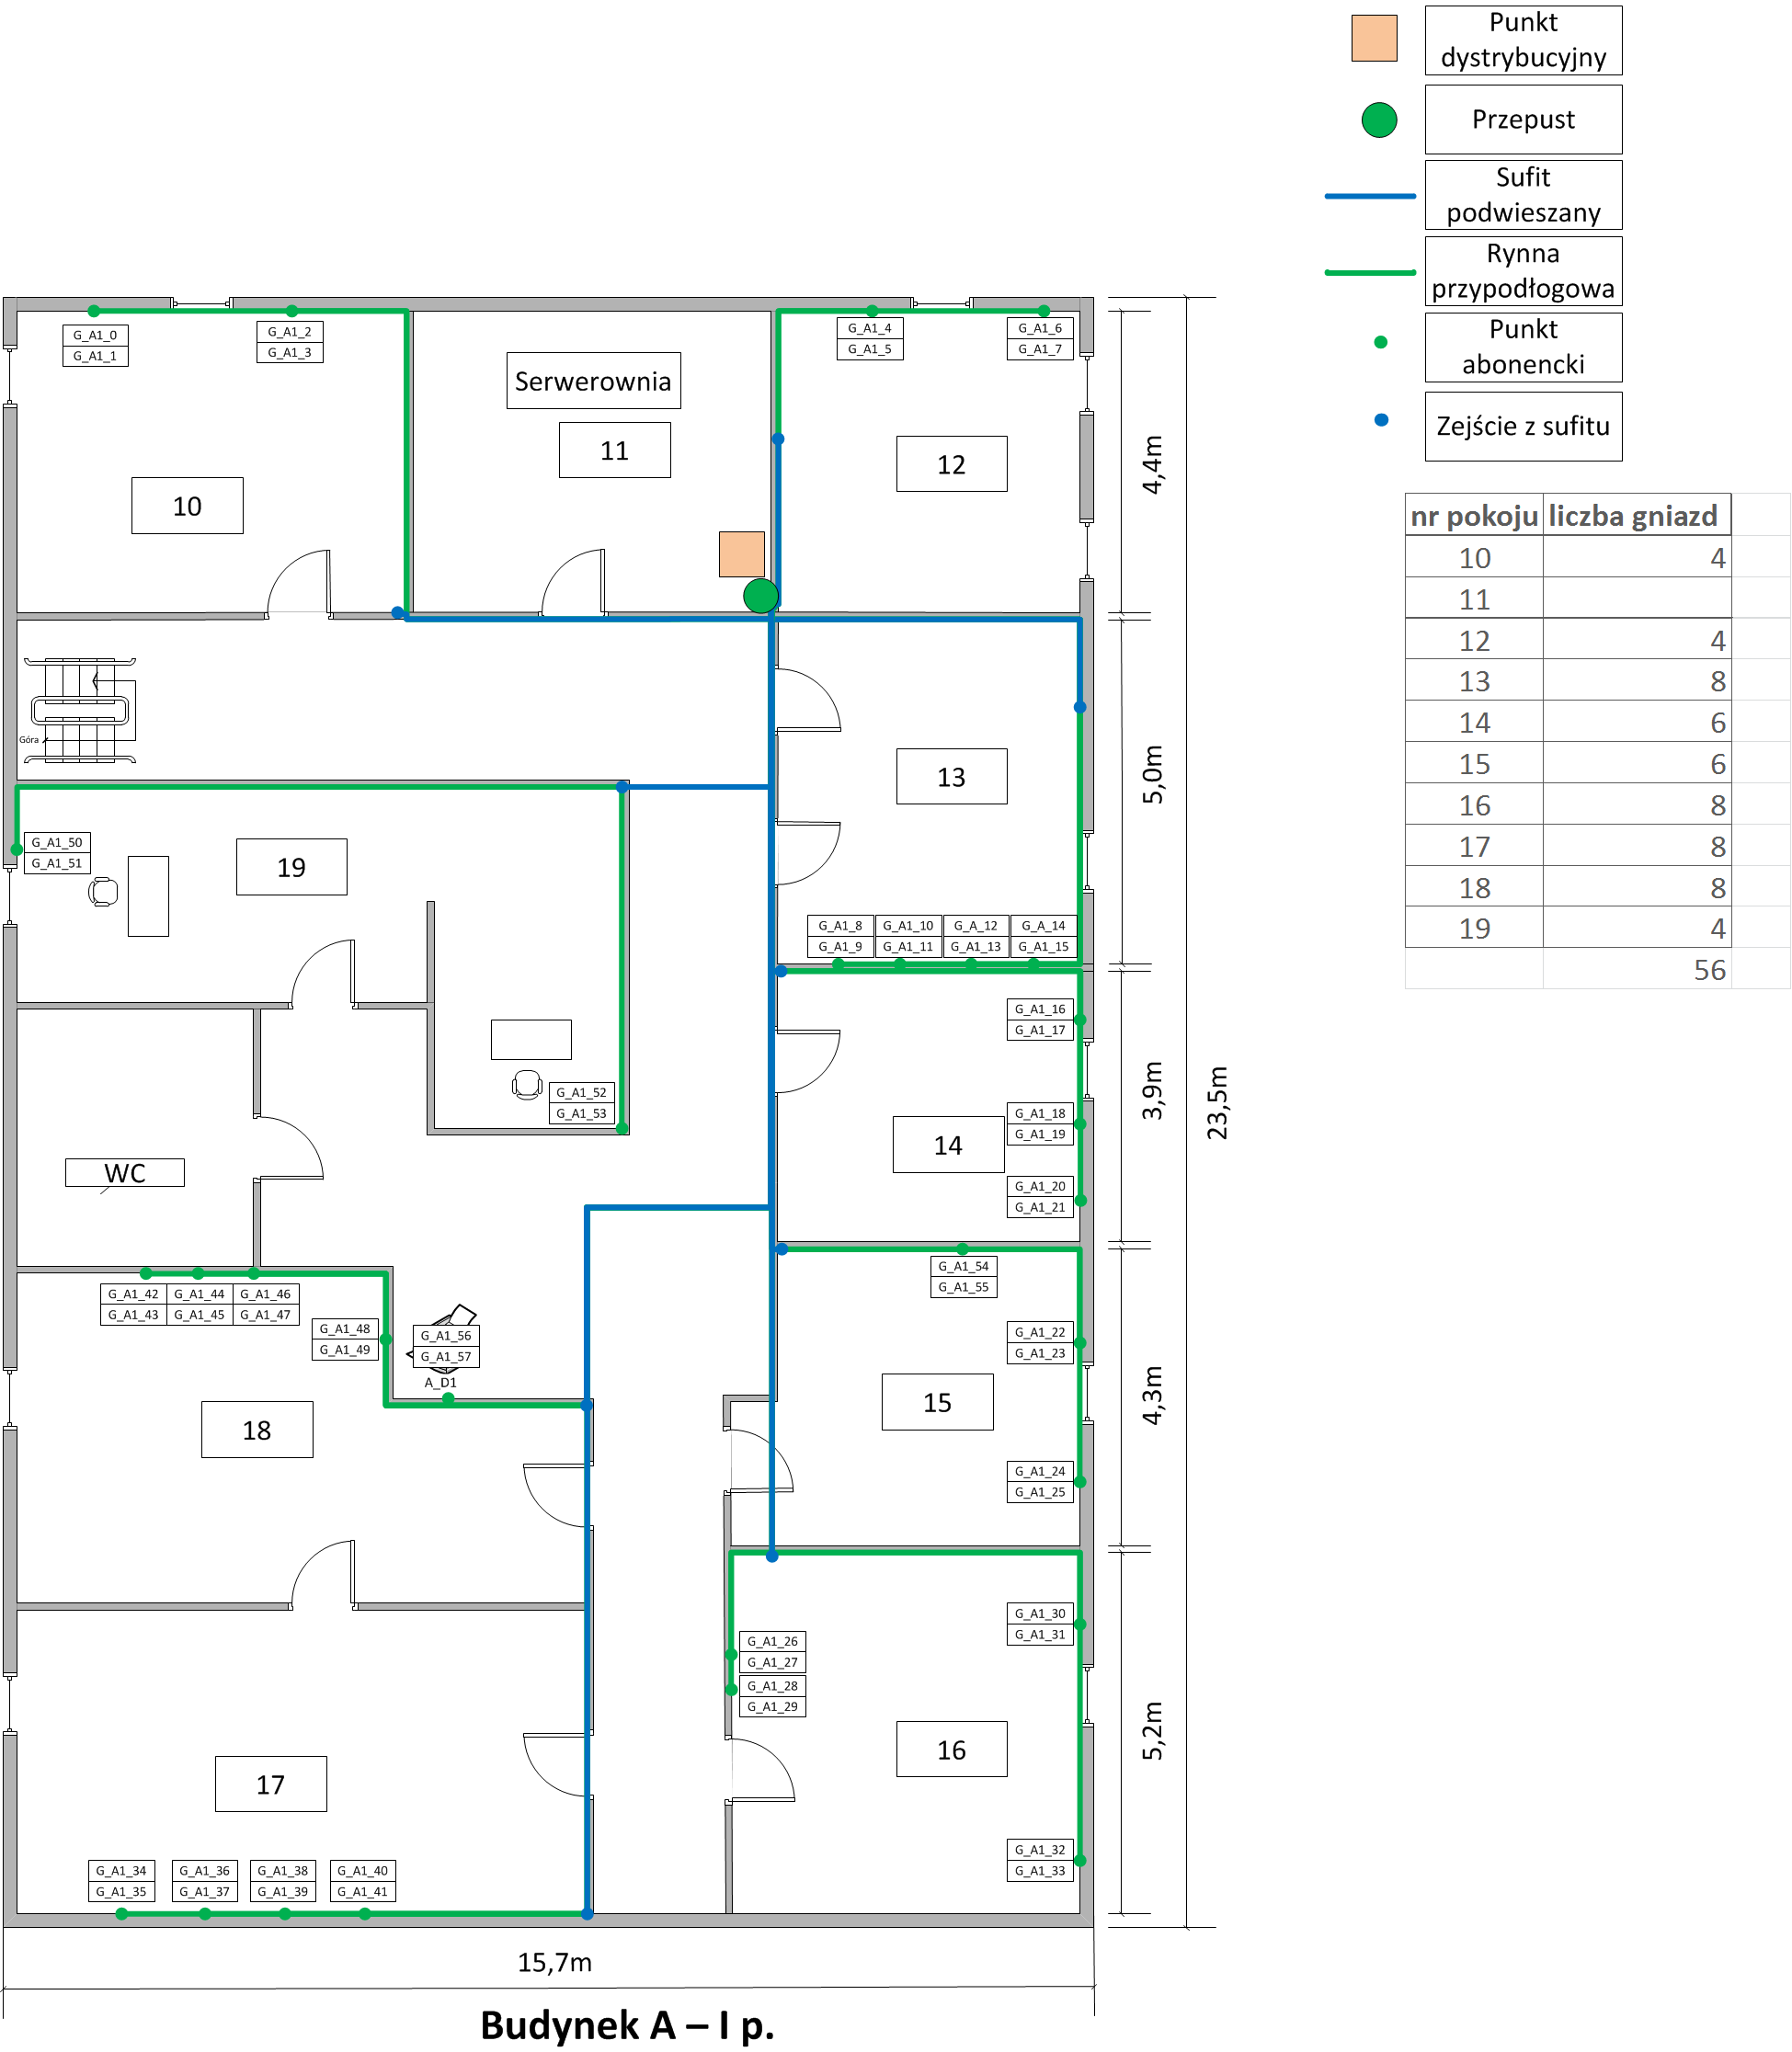
\includegraphics[width=\textwidth]{./obrazki/kable/a1.png}
  \caption{Projekt rozmieszczenia okablowania na 1 piętrze w budynku a.}
\end{figure}

\begin{figure}[H]
  \centering
      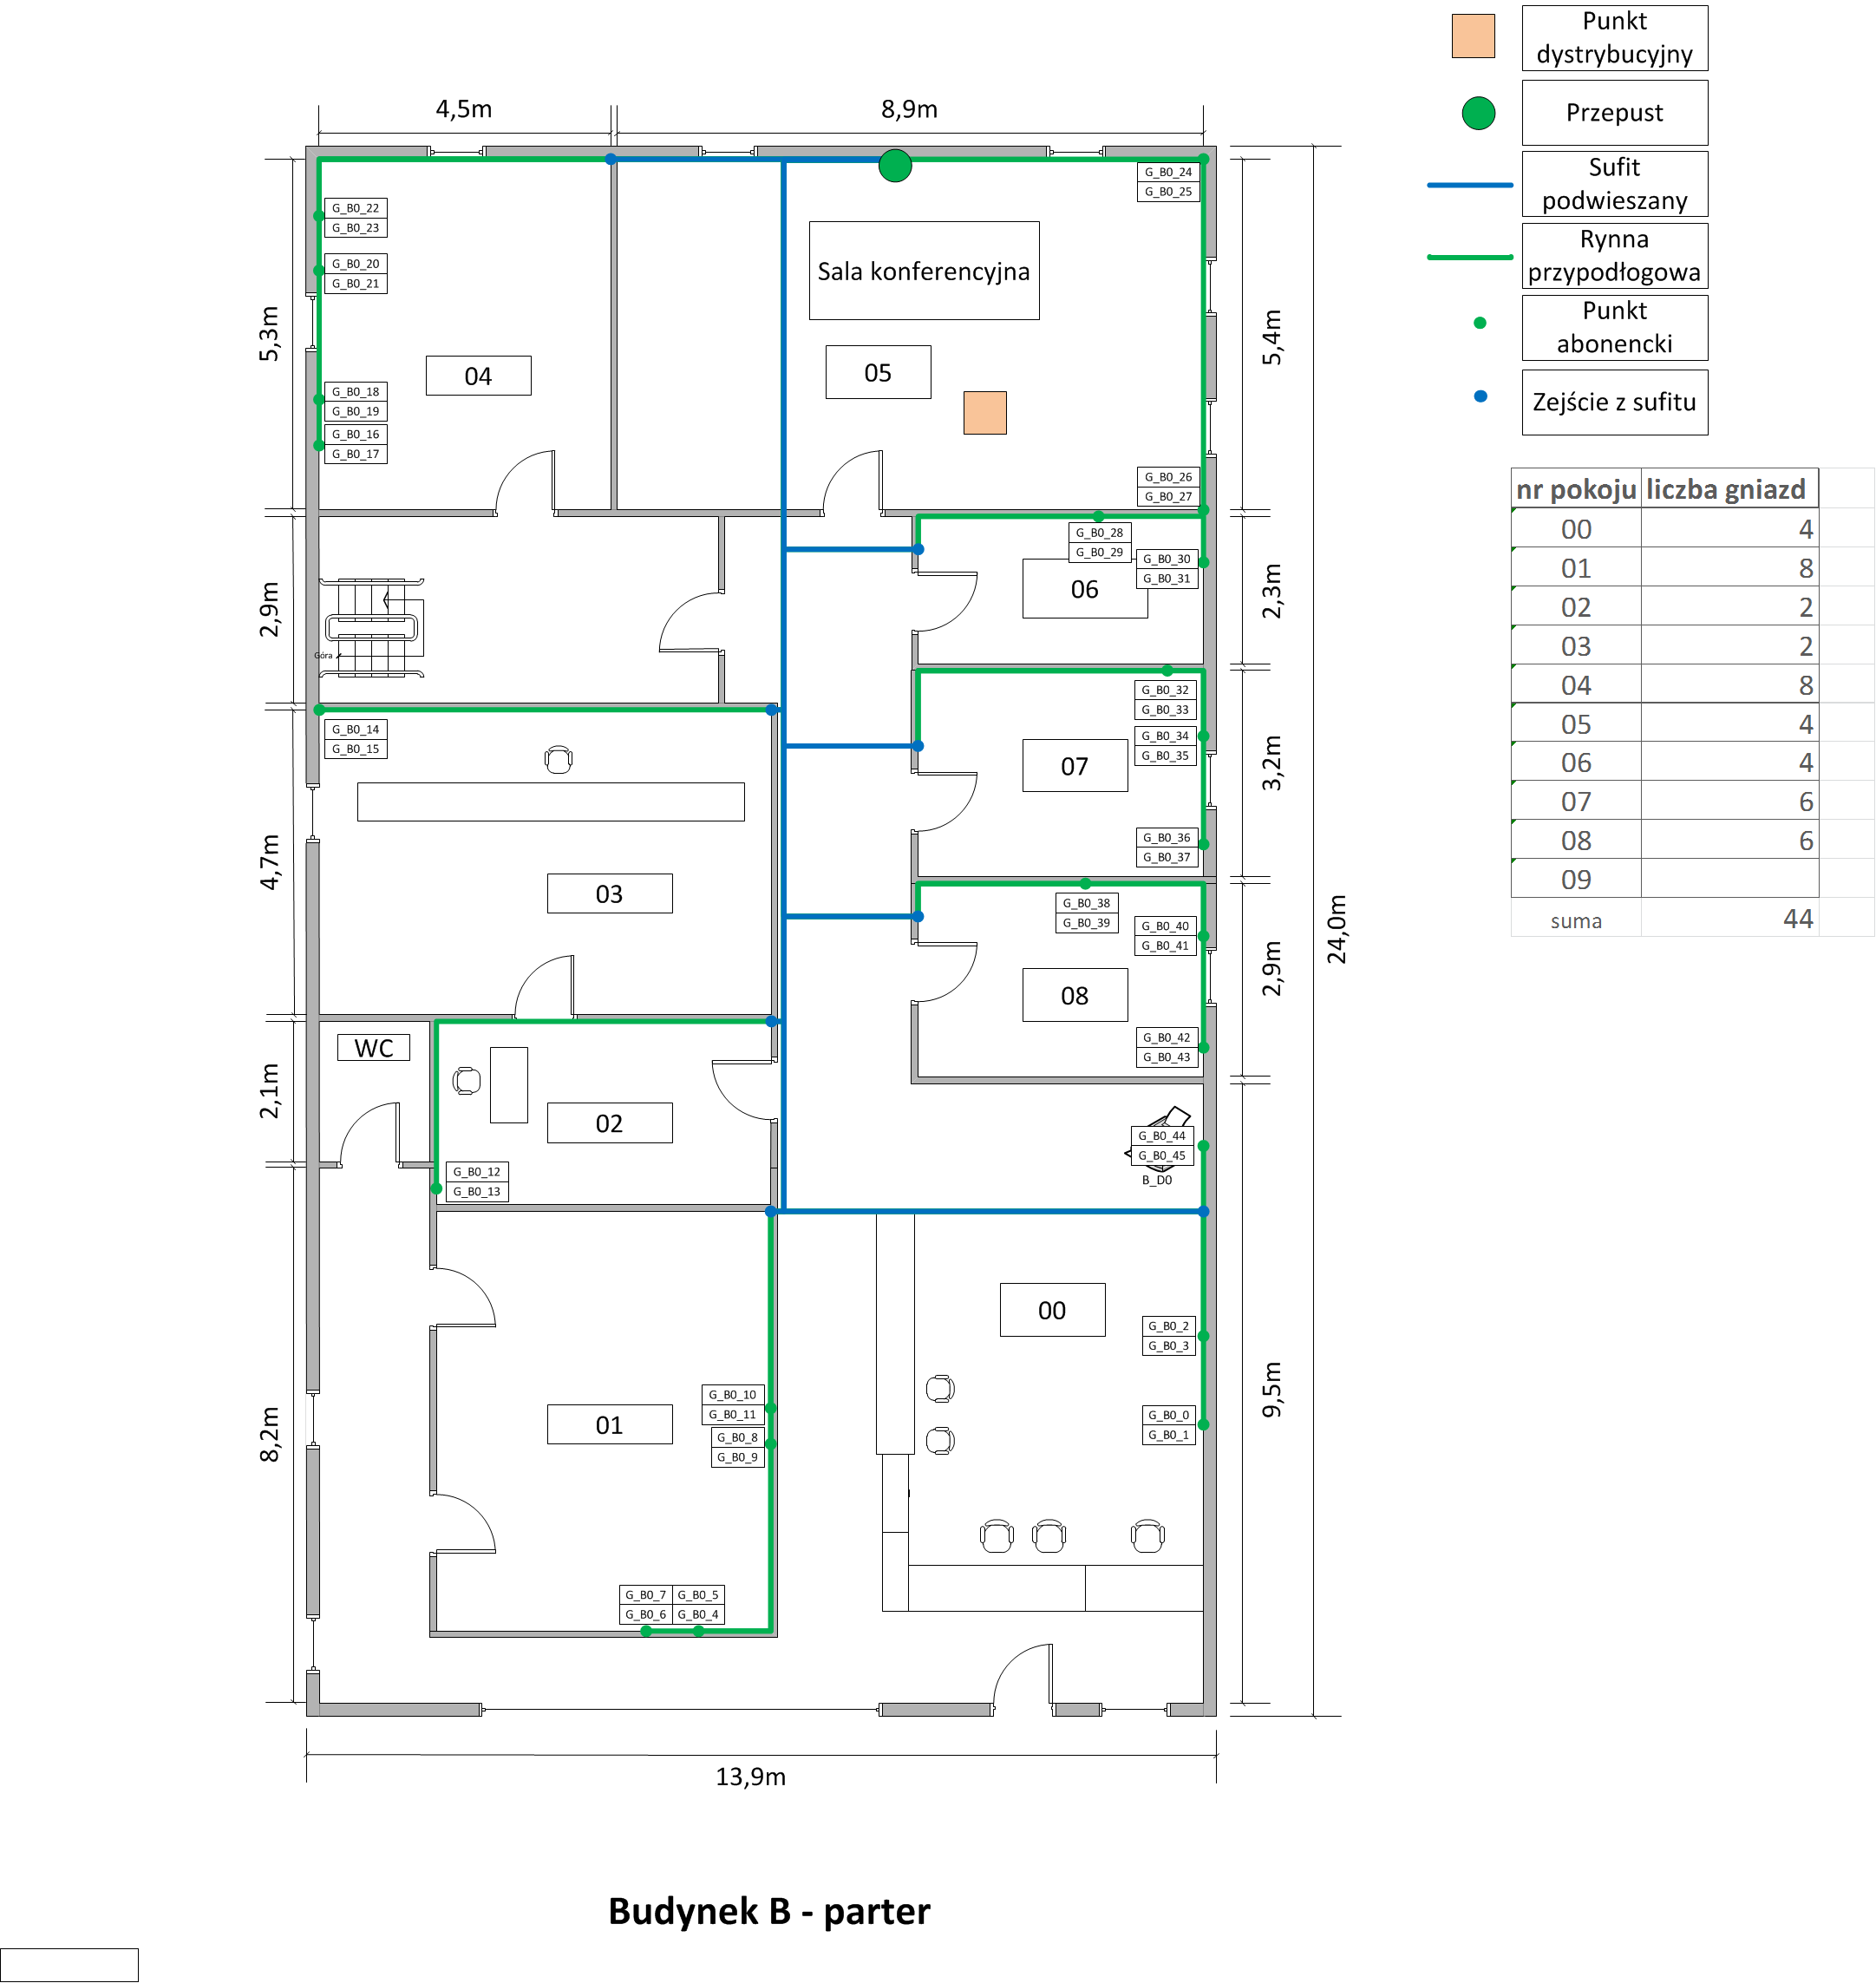
\includegraphics[width=\textwidth]{./obrazki/kable/b0.png}
  \caption{Projekt rozmieszczenia okablowania na parterze w budynku b.}
\end{figure}

\begin{figure}[H]
  \centering
      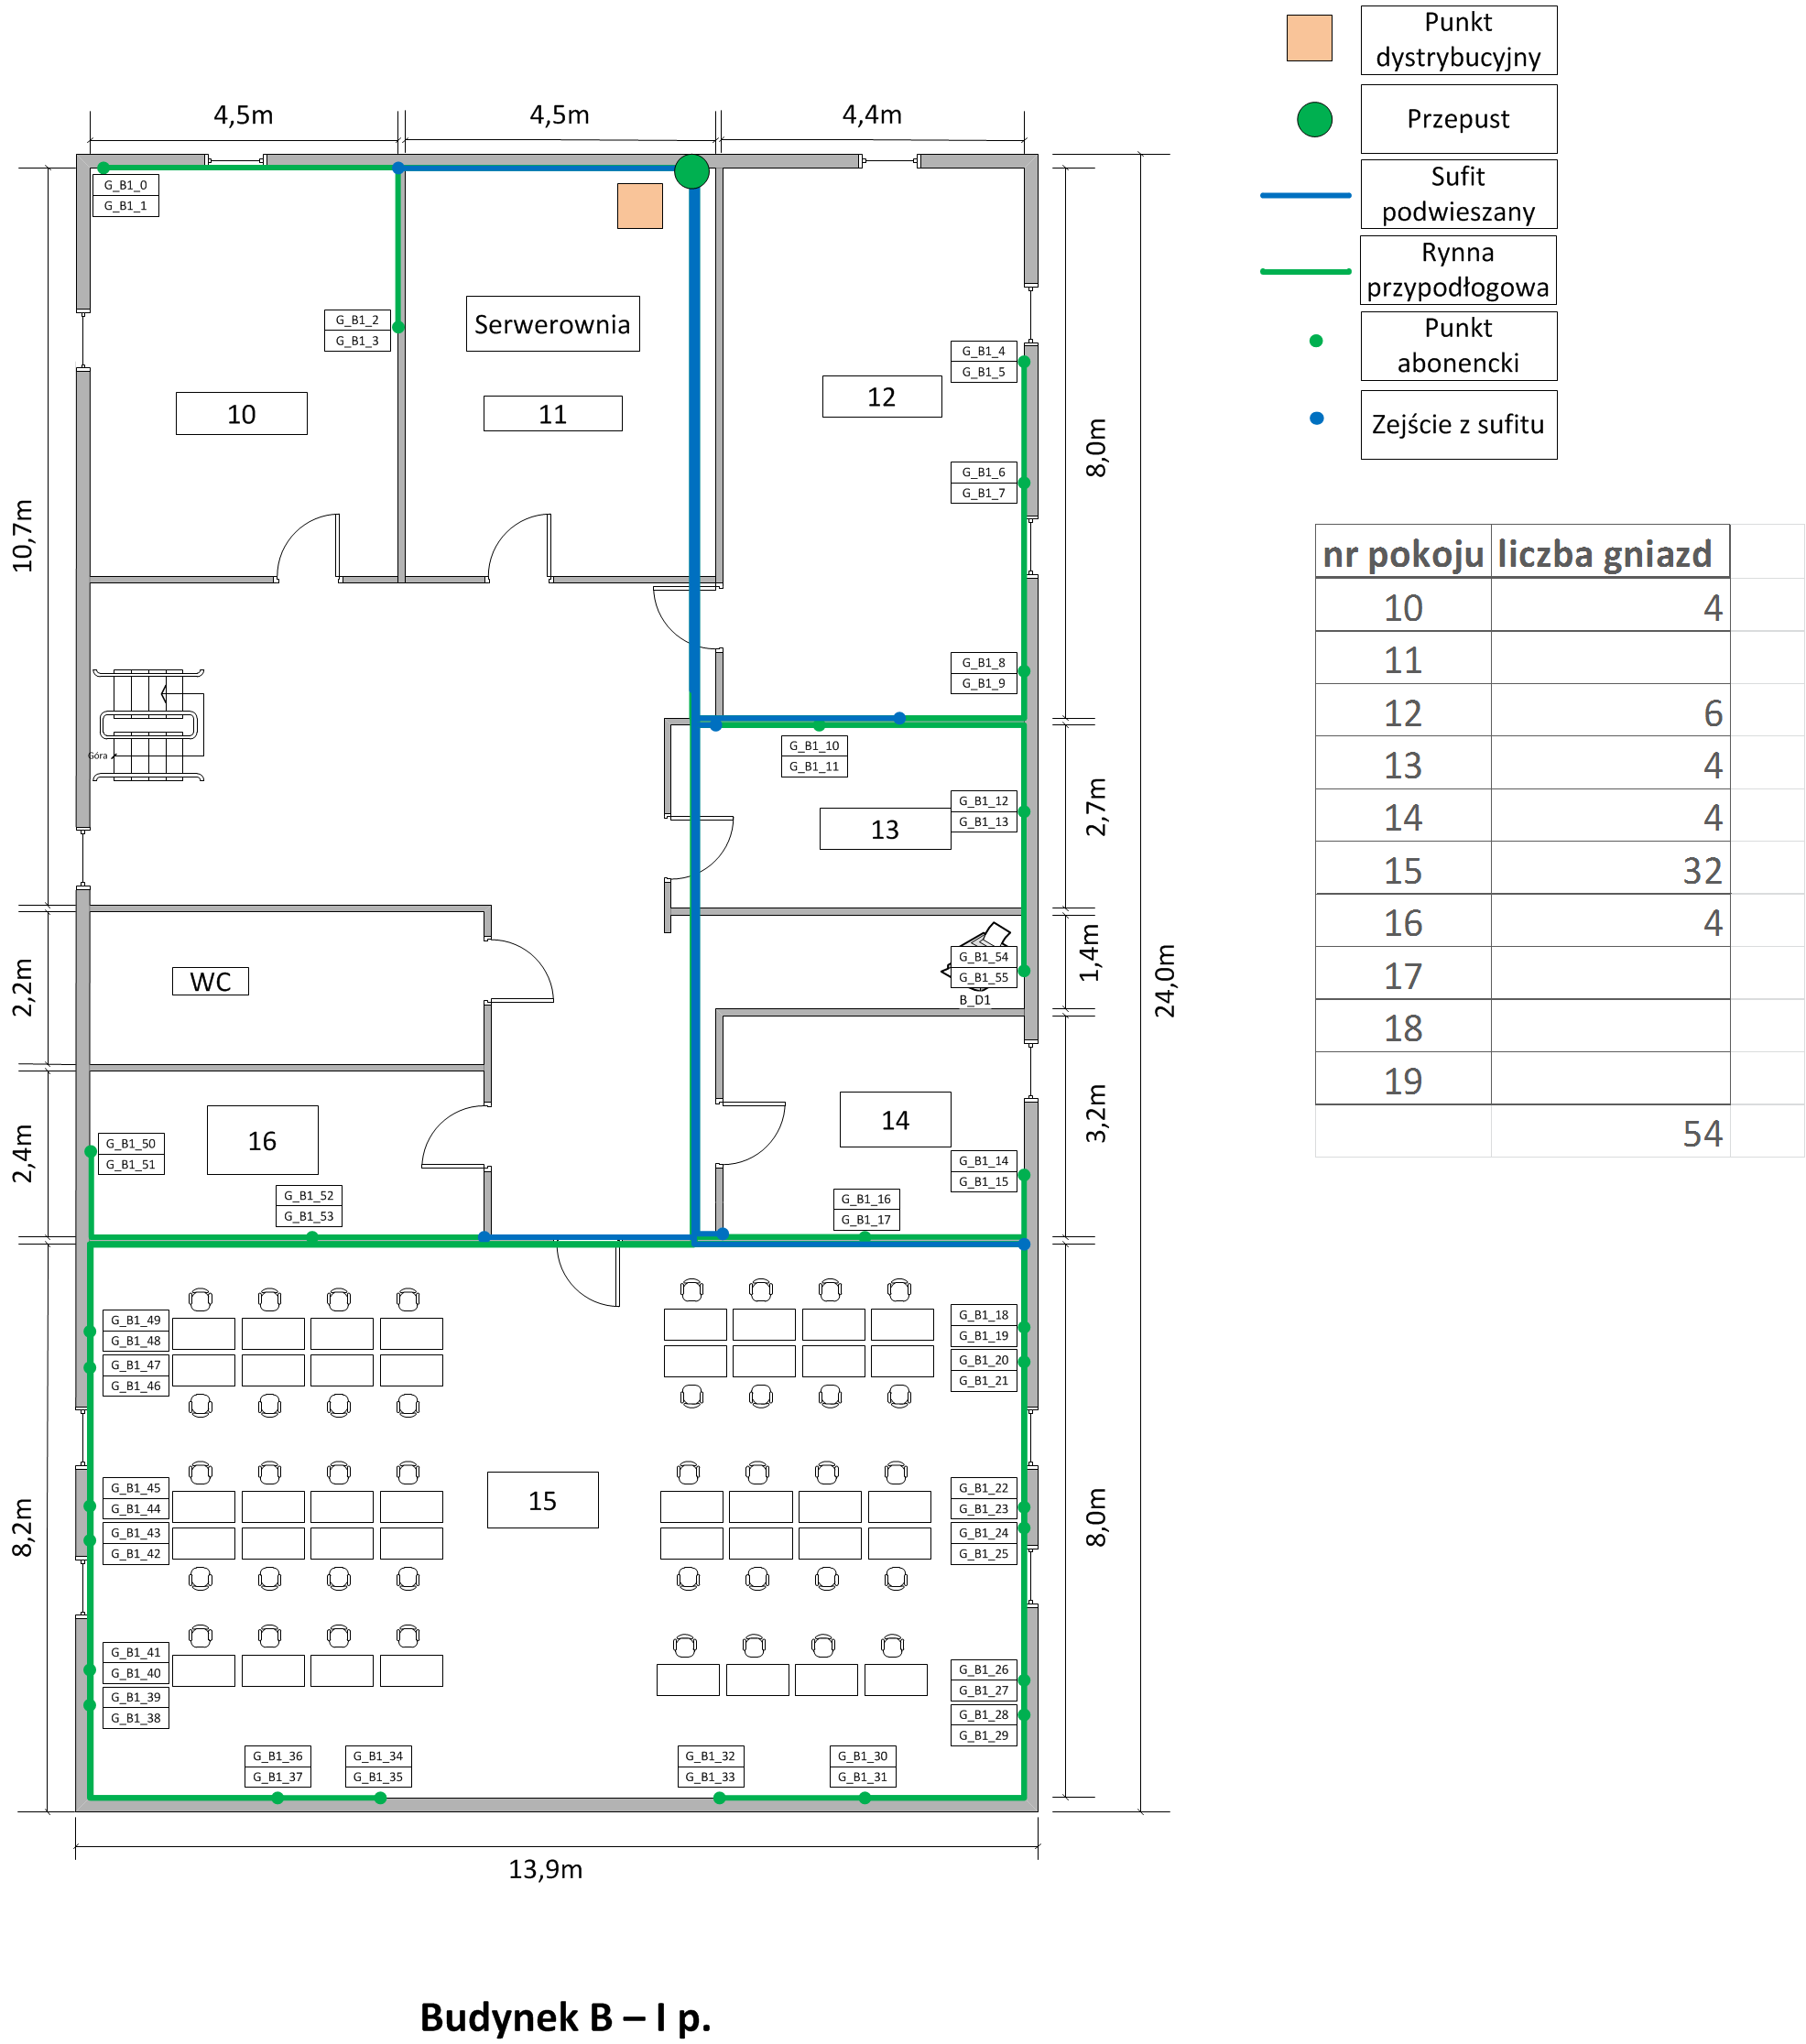
\includegraphics[width=\textwidth]{./obrazki/kable/b1.png}
  \caption{Projekt rozmieszczenia okablowania na 1 piętrze w budynku b.}
\end{figure}

\begin{figure}[H]
  \centering
      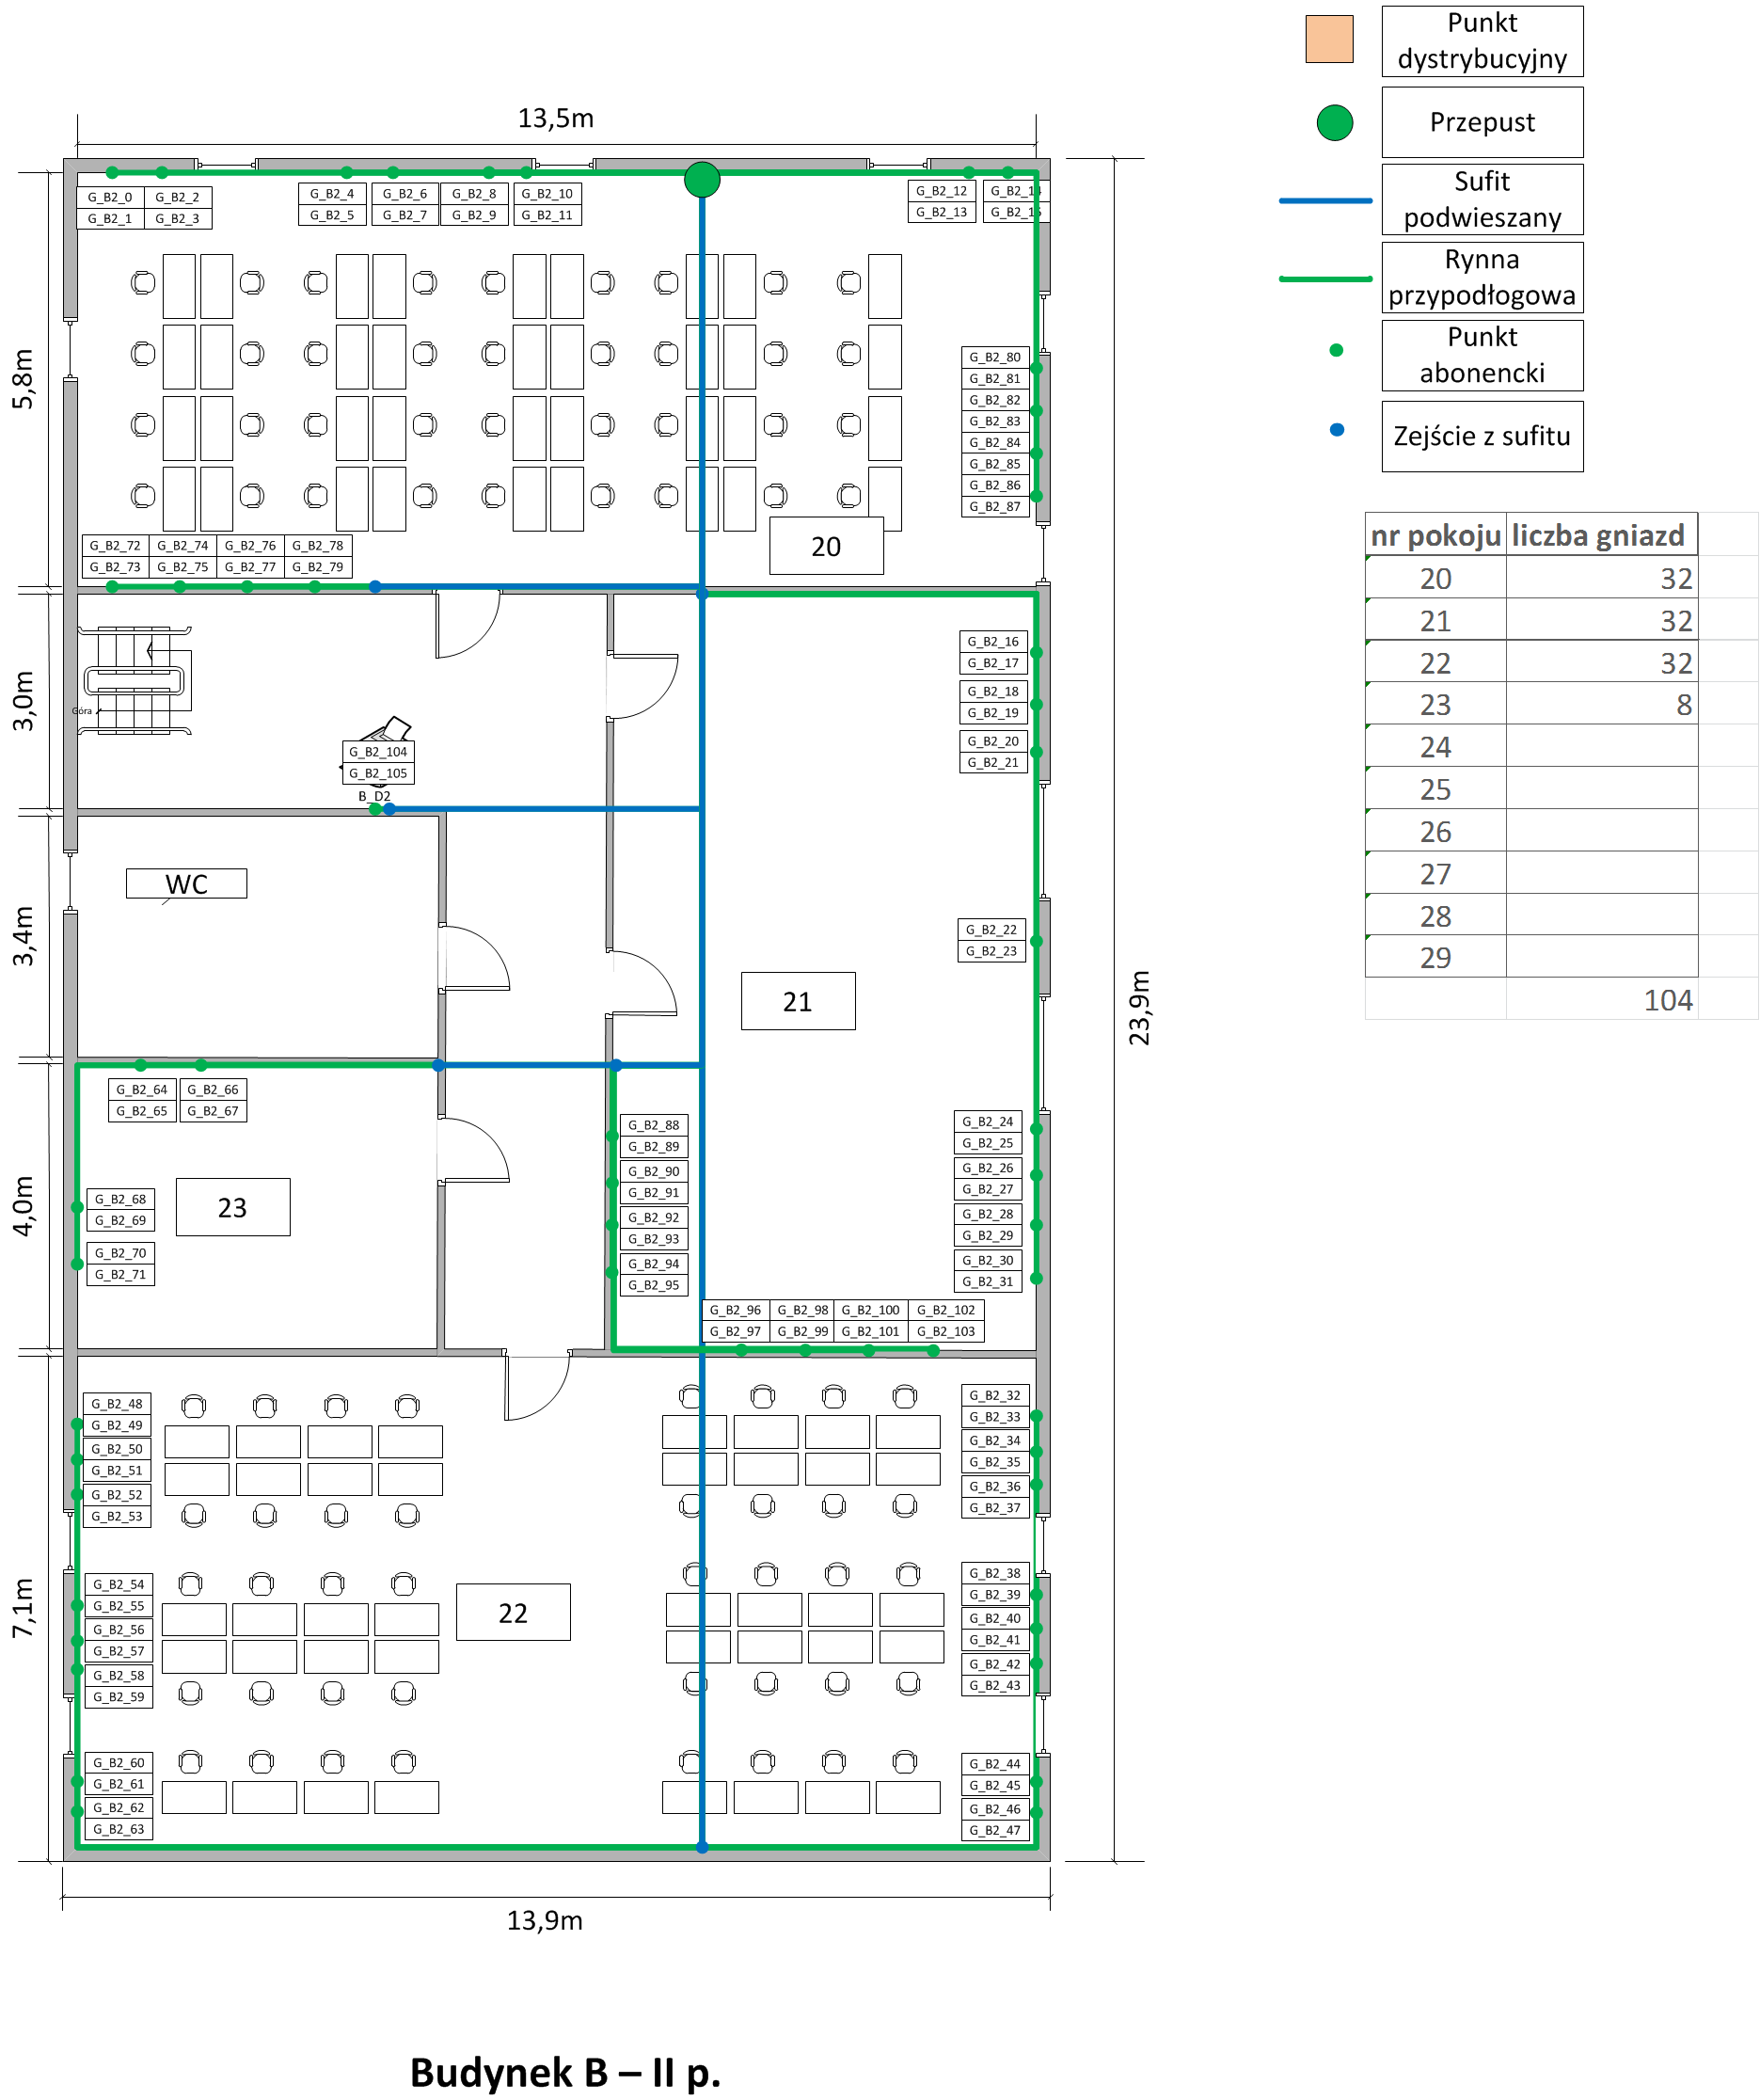
\includegraphics[width=0.9\textwidth]{./obrazki/kable/b2.png}
  \caption{Projekt rozmieszczenia okablowania na 2 piętrze w budynku b.}
\end{figure}


\subsection{Spis długości poszczególnych łącz}

\begin{table}[H]
\caption{Spis długości przewodów do poszczególnych punktów abonenckich na parterze w budynku a.}
 \centering
      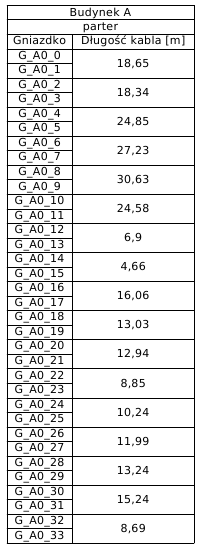
\includegraphics{./obrazki/dl_kable/a0.png}
\end{table}

\begin{table}[H]
\caption{Spis długości przewodów do poszczególnych punktów abonenckich na 1 piętrze w budynku a.}
 \centering
      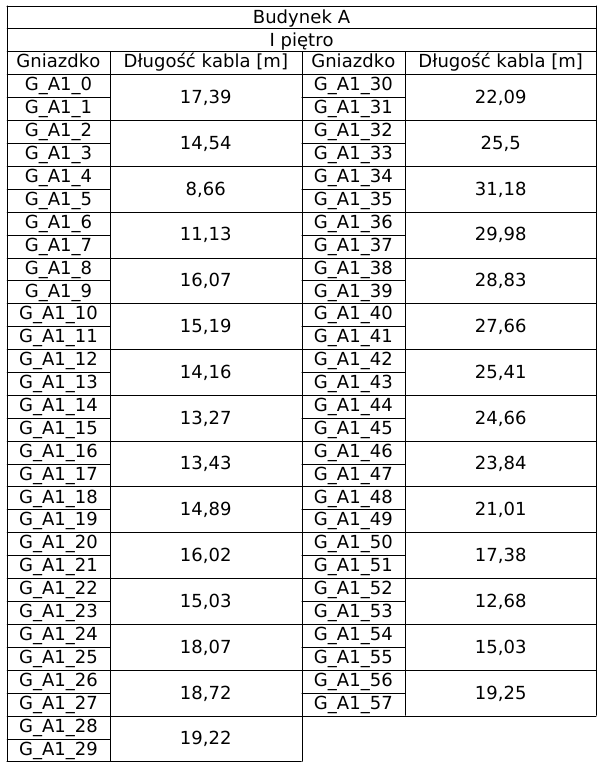
\includegraphics[width=0.8\textwidth]{./obrazki/dl_kable/a1.png}
\end{table}

\begin{table}[H]
\caption{Spis długości przewodów do poszczególnych punktów abonenckich na parterze w budynku b.}
 \centering
      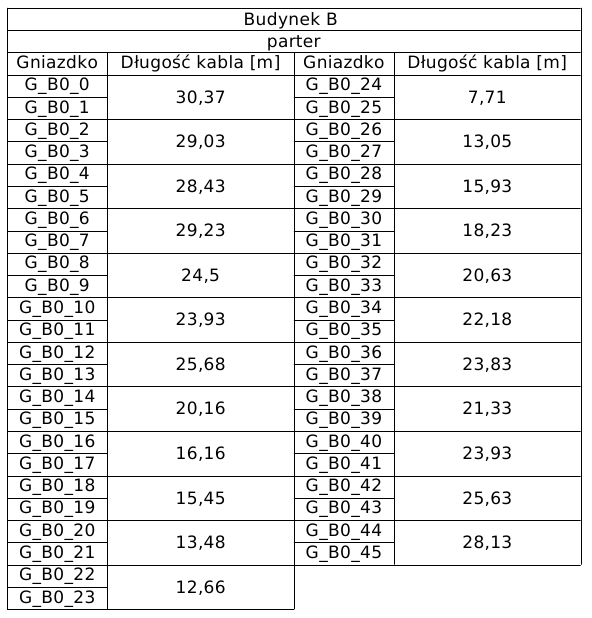
\includegraphics[width=0.8\textwidth]{./obrazki/dl_kable/b0.png}
\end{table}

\begin{table}[H]
\caption{Spis długości przewodów do poszczególnych punktów abonenckich na 1 piętrze w budynku b.}
 \centering
      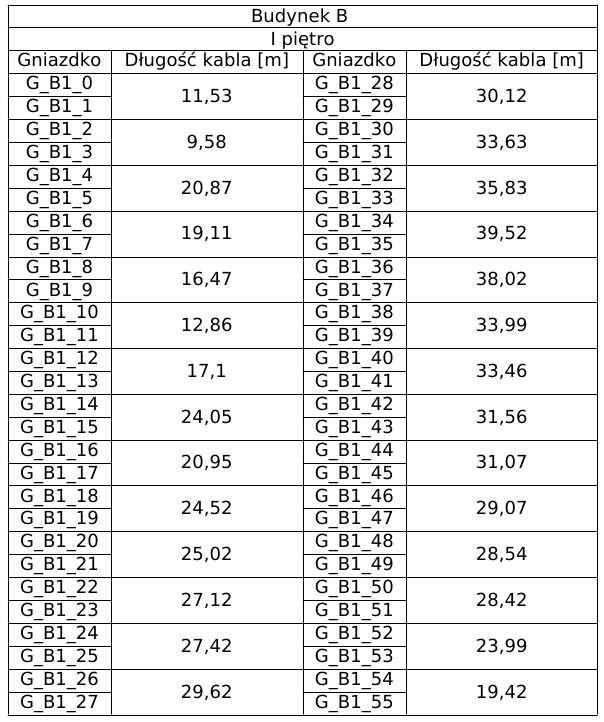
\includegraphics[width=0.8\textwidth]{./obrazki/dl_kable/b1.png}
\end{table}

\begin{table}[H]
\caption{Spis długości przewodów do poszczególnych punktów abonenckich na 2 piętrze w budynku b.}
 \centering
      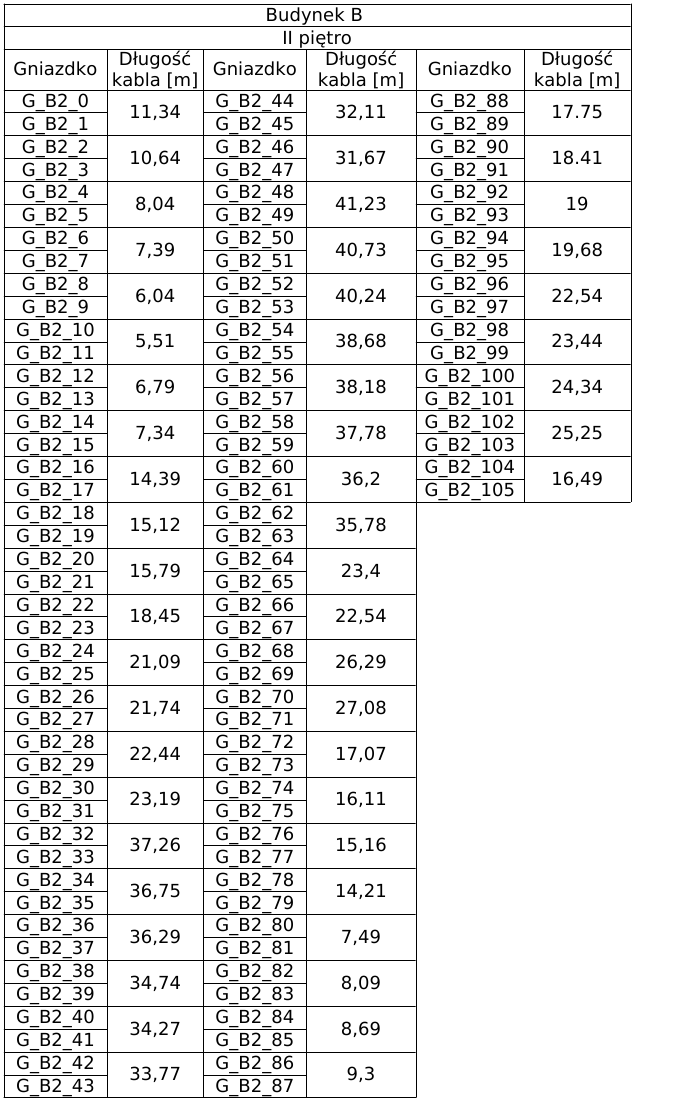
\includegraphics[width=0.8\textwidth]{./obrazki/dl_kable/b2.png}
\end{table}

\subsection{Przyporządkowanie interfejsów}

Switche są konstruowane z pomocą technologii stackable. Poszczególne moduły tego samego stosu są zaznaczone innymi kolorami.
Gniazda krosownic są przypożądkowane w taki sam sposób jak gniazda abonenckie do poszczególnych switchy.

\begin{table}[H]
\caption{Przyporządkowanie gniazd na parterze w budynku a do interfejsów switcha.}
 \centering
      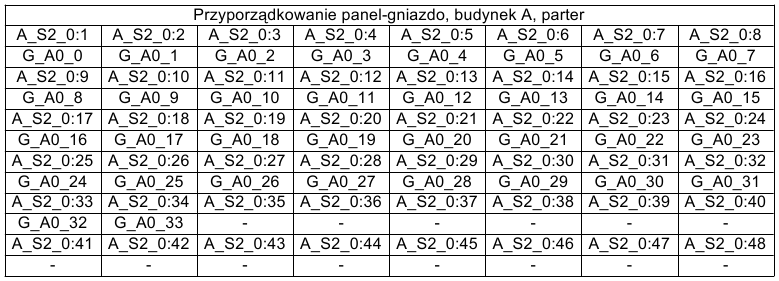
\includegraphics[width=0.8\textwidth]{./obrazki/tab_kros/a0.png}
\end{table}

\begin{table}[H]
\caption{Przyporządkowanie gniazd na 1 piętrze w budynku a do interfejsów switcha.}
 \centering
      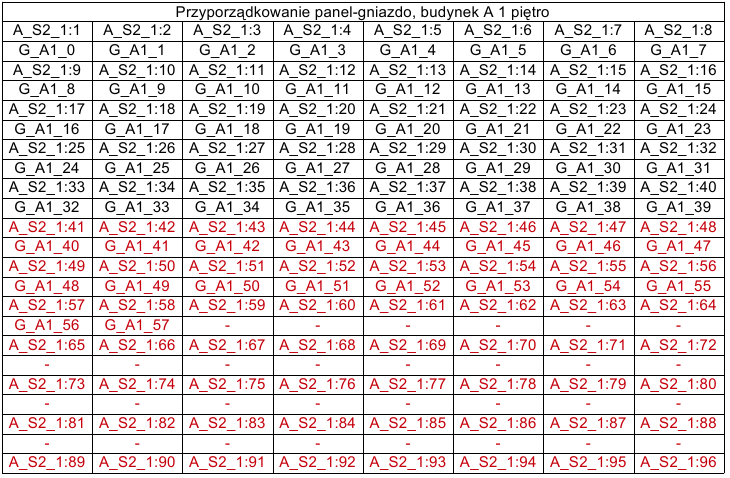
\includegraphics[width=0.8\textwidth]{./obrazki/tab_kros/a1.png}
\end{table}

\begin{table}[H]
\caption{Przyporządkowanie gniazd na parterze w budynku b do interfejsów switcha.}
 \centering
      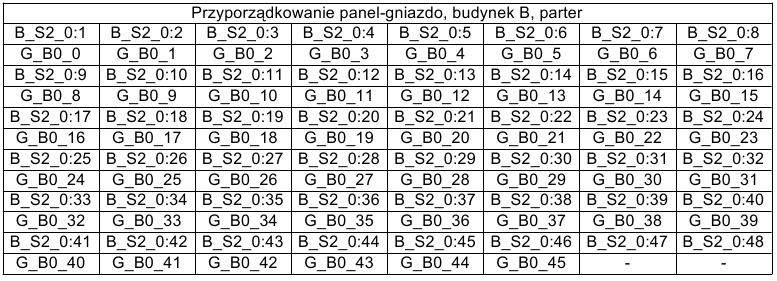
\includegraphics[width=0.8\textwidth]{./obrazki/tab_kros/b0.png}
\end{table}

\begin{table}[H]
\caption{Przyporządkowanie gniazd na 1 piętrze w budynku b do interfejsów switcha.}
 \centering
      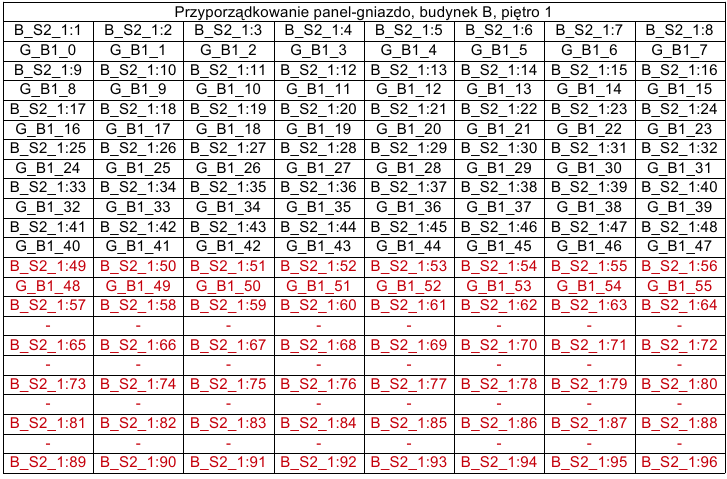
\includegraphics[width=0.8\textwidth]{./obrazki/tab_kros/b1.png}
\end{table}

\begin{table}[H]
\caption{Przyporządkowanie gniazd na 2 piętrze w budynku b do interfejsów switcha.}
 \centering
      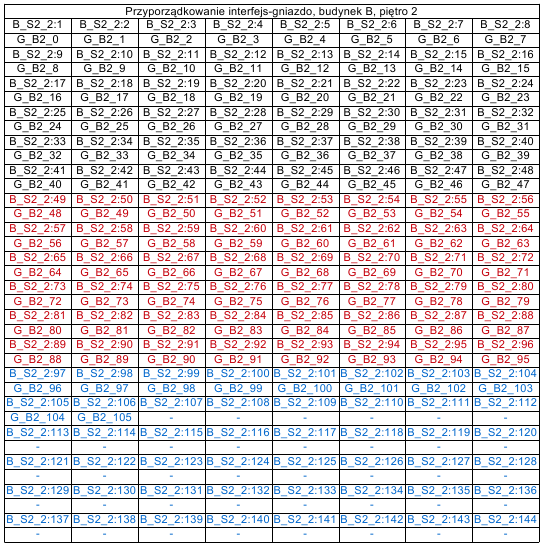
\includegraphics[width=0.8\textwidth]{./obrazki/tab_kros/b2.png}
\end{table}

\begin{table}[H]
\caption{Przyporządkowanie gniazd w A\_S3}
 \centering
      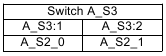
\includegraphics{./obrazki/tab_kros/as3.png}
\end{table}

\begin{table}[H]
\caption{Przyporządkowanie gniazd w B\_S3}
 \centering
      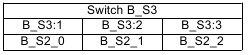
\includegraphics{./obrazki/tab_kros/bs3.png}
\end{table}

\begin{table}[H]
\caption{Przyporządkowanie gniazd w B\_R\_0.}
 \centering
      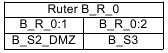
\includegraphics{./obrazki/tab_kros/br0.png}
\end{table}


\subsection{Rozmieszczenie urządzeń w szafach RACK}

\begin{figure}[H]
  \centering
      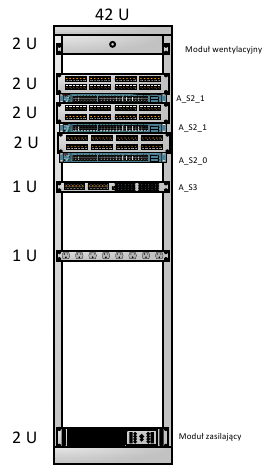
\includegraphics[width=0.5\textwidth]{./obrazki/rack/a.png}
  \caption{Projekt rozmieszczenia modułów w szafie RACK dla budynku a.}
\end{figure}

\begin{figure}[H]
  \centering
      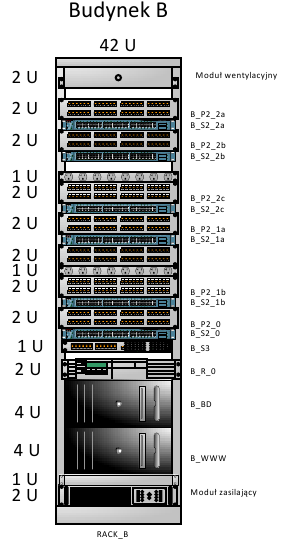
\includegraphics[width=0.5\textwidth]{./obrazki/rack/b.png}
  \caption{Projekt rozmieszczenia modułów w szafie RACK dla budynku b.}
\end{figure}

\section{Projekt podłączenia do Internetu}

Sieć wewnętrzna zostanie połączona z internetem za pomocą
dwóch łączy. Będą one posiadały identyczne parametry aby w razie awarii jednego z nich praca firmy została niezakłócona. Łącza te zostaną
zapewnione przez firmę SEEV. Witrynę firmy można znaleźć pod adresem internetowym \url{http://www.seev.pl}.

O wyborze tej firmy w głównej mierze zdecydowały
możliwość zamówienia łącza o wysokich przepustowościach oraz możliwość dopasowania oferty do indywidualnych potrzeb.
Ponadto firma ta świadczy usługi na terenie Wrocławia. 

Po uwzględnieniu wymagań narzuconych przez zaprojektowaną sieć oraz wytycznych określonych przez klienta, każde
z dwóch zamówionych łączy będzie miało następującą specyfikację:
\begin{itemize}
 \item Pobieranie: 40 Mb/s
\item Wysyłanie: 40 Mb/s
\item Typ łącza: symetryczne
\item Interfejs podłączenia: SC/APC światłowód
\item Limit danych: brak
\item Gwarancja przepustowości: zapewniona

\end{itemize}

Dodatkowo firma SEEV zapewnia następujące parametry niezawodnościowe zawarte w certyfikacie SLA:
\begin{itemize}
\item gwarantowany czas reakcji na awarię 30 minut
\item czas naprawy łącza 24h
\item dostępność sieci SEEV w skali roku 99,9%.
\end{itemize}


\section{Analiza bezpieczeństwa i niezawodności sieci}
Sieć komputerowa narażona jest na szereg niebezpieczeństw.Zaczynając od 
najprostszych awarii sprzętu a kończąc na celowym ataku na infrastrukturę i dane biznesowe.
Proponowany przez nas projekt sieci zapewnia dodatkową odporność na następujące zagrożenia:
\begin{itemize}


\item{Złośliwe oprogramowanie}

Pierwszą linią obrony jest użycie ściany ogniowej
w routerze podłączonym do internetu a urządzeniami pośrednimi oraz
końcowymi. Kolejnym  zabezpieczeniem
jest użycie sieci wirtualnych VLAN. Uniemożliwiają one rozprzestrzenienie się złośliwego oprogramowania na całą sieć.           

Powyższe zabezpieczenia nie zwalniają firmy z obowiązku korzystania z 
aktualnych programów antywirusowych oraz szkolenia pracowników na temat zagrożeń w sieci.

\item {Ataki oraz włamania do sieci}

Po raz kolejny pierwszą linią obrony jest zapora ogniowa,
która może zabronić dostępu do sieci informacjom podejrzanym lub
szkodliwym. 

Kolejnym mechanizmem obronnym w tym przypadku jest strefa zdemilitaryzowana w której umieszczono serwer www.
Mimo, że  włamanie zakończy się sukcesem to nie wiąże się z
narażeniem firmy na penetracje wewnętrznych zasobów i znaczące straty.

\item {Zabezpieczenie sieci  WiFi}

W celu zapewnienia jak największego bezpieczeństwa sieci
WiFi, na terenie firmy, wprowadzono potrzebę autentykacji
użytkownika przez podanie hasła podczas logowania. Transmisja będzie szyfrowana za pomocą metody WPA2 Enterprise.

Dodatkowo zmniejszenie mocy sygnału sieci do poziomu umożliwiającego korzystanie z niej tylko w obrębie budynku
uniemożliwi osobom postronnym podsłuchiwanie transmisji.

\item Awaria Zasilania.

Sieć stworzona na potrzeby firmy wymaga do działania energii
elektrycznej i jest od niej całkowicie zależna. Aby przeciwdziałać skutkom braku energii,zaleca się zakup zasilaczy UPS.
Umożliwią one bezpieczne wyłączenie serwerów bez utraty danych. Informację przechowywane lokalnie na
każdym z komputerów nie podlegają takiej ochronie.

\item {Awaria serwerów}

Aby zapobiec trwałej utracie danych, każdej doby, w godzinach nocnych firma wykonuje backup bazy danych na
zewnętrzne serwery.Zalecane są również prace serwisowe na  sprzęcie
mają zminimalizować ryzyko wystąpienia awarii nośników danych.

\item {Zakłócenia EMC}

Mimo że środowisko EMC w którym znajduje się firma nie jest zbytnio zanieczyszczone należy zastosować środki zapobiegawcze
aby sieć mogła służyć zamawiającemu przez długi czas.Sprzęt użyty do
stworzenia sieci lokalnej firmy oraz okablowanie musi spełniać wszystkie normy ISO
oraz pochodzić od sprawdzonej firmy.

Najbardziej narażonym na zakłócenia jest zewnętrzny odcinek sieci poprowadzony między budynkami. W dodatku jest to krytyczne miejsce. 
Aby zapewnić maksimum ochrony w projekcie użyliśmy najbardziej odpornego na zakłócenia medium czyli światłowodu.


\item {Ograniczenia dostępu fizycznego do urządzeń}

Pomieszczenie, które wybraliśmy do umieszczenia sprzętu sieciowego jest specjalnie przystosowane.
Zamknięte jest za pomocą solidnych drzwi z skomplikowanym zamkiem ponadto nie posiada okna. Chłodzenie jest w nim
realizowane za pomocą specjalnej wentylacji.Dodatkowo urządzenia zamontowane są w szafach zamykanych na klucz. 
Dostęp do nich posiadają jedynie autoryzowane osoby.

\end{itemize}

\section{Kosztorys urządzeń}

\begin{table}[H]
\caption{Koszty comiesięczne ponoszone przez firmę.}
\label{table:koszty_loncze}
 \centering
      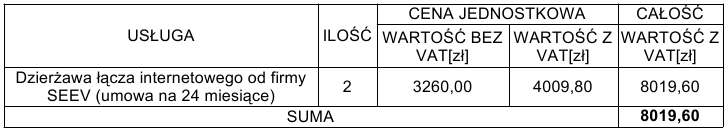
\includegraphics[width=0.8\textwidth]{./obrazki/koszty/koszty_loncze.png}
\end{table}

%Otoczenie tabelki
%\begin{table}
 % \caption{Geograficzne rozmieszczenie odziałów firmy.}
 %\includegraphics[width=0.9\textwidth]{./obrazki/topologia.jpeg}
%\end{table}

%\begin{figure}[h!]
 % \centering
 %     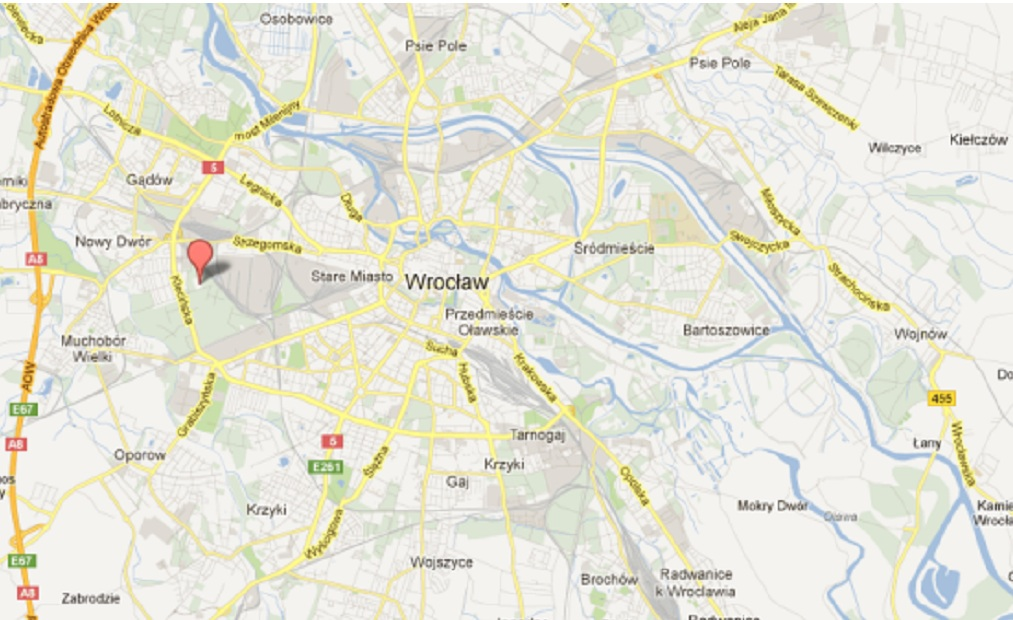
\includegraphics[width=0.9\textwidth]{./obrazki/adres_computerbudy.jpeg}
%  \caption{Geograficzne rozmieszczenie odziałów firmy.}
%\end{figure}
\begin{enumerate}
 \item Dodać na opisie tabelek połączeń że gniazdko do panela krosowniczego tak samo 1:1- zrobione (Gniazda krosownic są przypożądkowane w taki sam sposób jak gniazda abonenckie do poszczególnych switchy.)
\item Zaznaczyć na rysunkach szaf rakowych który switch jest który tak aby nie było niedomówień.
\end{enumerate}

 


\end{document}
